\chapter{Control in the Platform economy: The case of New York City}

To this point we have provided tools in which to measure the power of nodes and affiliations within a weighted aspectual hypergraph. These measures make use of both the structure of the hypergraph, the projected networks that emerge, and the value attached to certain affiliations. Although the measures are created in an abstract fashion, they have direct application to directorate hypergraphs. Specifically, nodes can be represented as directors and affiliations can be represented by firms such that the value of an affiliation is given by the book value of their assets, or capital stock. Assuming that each director has equal voting rights on the policies of the firm that they are a member of, the (weighted) $\sigma$-score can be appropriately used to measure the influence of individual directors on the policies of the set of firms that they are directors of. A director can therefore increase their $\sigma$-score by becoming a member of firms with fewer other directors in which to share voting rights, and/or by becoming a member of a set of firms with a higher value attached to them. This application is discussed in Section~\ref{Application:Network} below.

\paragraph{Chapter outline.}

Section~\ref{Application:Network} assesses the structure of the directorate network of New York City, providing an analysis of the elite network structure and centralisation of power. Specific focus is paid to the Northern Securities Company. Section~\ref{Application:Regression} provides an econometric analysis regarding the relationship between proposed measures of influence, centrality, and the economic performance of the firm. The final section concludes and provides future areas of research.

\section{Influence, elites, and the rise of the Empire State} \label{Application:Network}

We apply the measures of hypergraph centrality and the notion of elites to the directorate of New York City in 1902. We consider the network of directors as a weighted aspectual hypergraph whereby aspects correspond to the distinct industries that firms are considered to operate in. An individual is a member of an aspect if they are the director of a firm that operates in that aspect.

We use a historic application for multiple reasons. The first is due to the interesting time period as discussed in the introductory section of this chapter. Indeed, we noted the particular interest of spanning interlocking directorates during this time by Government leading to institutional changes. Second, due to more practical reasons regarding the assignment of aspects and computation. Within modern economies conglomerates---firms that operate in many different industries---exist and can therefore operate in many different aspects thus complicating the analysis; however these were not seen to be of any significance during the time period assessed. The historical data here thus provides the advantage of a much simpler economy in which to apply the measures of centrality and influence discussed above\footnote{Future research may focus on more contemporary economies. However, the sheer size of the network and institutional and organisational complexity inherent within modern directorate networks may lead to difficulty in parsing out useful information.}.

When considering directorship networks there exists a set of firms, which are equivalent to the set of affiliations, and a set of directors, which are equivalent to the set of nodes, as described above. Firms are partitioned into different aspects depending on the industry that they operate in as indicated by the \emph{Directory of Directors of New York City}.

The empirical study takes into consideration three industries that are known to be of importance in New York City in 1902, these are: (1) banking and trusts, (2) railways and railroads, and (3) insurance. The reason these industries were chosen was due to the known integration of finance and railroad transport during this time. During the beginning of the 20th Century it was continually speculated that control between the railroad and financial industries were becoming more concentrated in the hands of a few known financiers (New York Times, 1902a). Moreover, as noted above, a case of potential monopolisation was brought to court regarding the establishment of the National Securities Company (New York Times, 1902b).

Prior to 1914 there existed no restrictions regarding the make-up of firm directorates in America. This largely unrestricted formation of directorates suggests that directors will connect to firms that are, in some way, complementary. Thus, the existence of directors in multiple aspects suggests that there must exist some complementarity between aspects as there is something to be gained from being embedded in these aspects. This is reflected in a smaller distance between aspects.

The search for elites is also applicable here for two reasons. First regards the ``old boy'' nature of the directorate network during this time. It has been noted that there existed assortivity between directors, which suggests that there was an increased tendency for directors to be board members of the same set of firms when they were already members of at least one firm together, thus indicating nepotism in the directorship network. Due to this nepotism we would find that there would be an increased tendency for elite nodes to be connected to one another, thus forming more integrated networks. Second is the claim that there existed some control of directors that spanned multiple industries. As noted in the introduction, Morgan and others were considered to be influential players in the evolution of multiple industries, including banking and trusts, insurance, and railways, with widely spanning social and economic ties throughout the economy (Pan, 2012).

The layout of this section is as follows. First, we assess the context of the directorate network and provide summary statistics regarding the networks' structure and the aspectual distance between industries. Second, we introduce our proposed measures of centrality and influence, identifying elites, and analysing brokerage opportunities in this network. This assessment sets up the econometric analysis regarding the relationship between the centrality and influence of financial institutions and the economic performance of the firms.

\paragraph{Directorate data.}

The network data used is collected from the \emph{Directory of Directors in New York City} over this time period. This directory provides the population of directors and firms in the New York area. Note however, that although the network is extremely well populated it may not be fully because some directors, and the companies they are directors of, may be situated in other parts of the world. For example, Chicago and California contain many directors that are in positions in New York companies considered.

\subsection{Overview of the directorate hypergraph}

Financial institutions placed directors on the board of other financial institutions and firms that they were heavily indebted in (Pujo Committee, 1913). This makes the directorate membership network of New York City a proxy for closeness of cooperation between financial institutions and firms during this time. There are a number of immediate effects of such relationship building:
\begin{abet}
\item[(1)] To coordinate interest rates given to borrowers; and
\item[(2)] To call upon others for favours.
\end{abet}
The second effect is particularly relevant when considering the coordinated private bailout of firms during the Bankers Panic of 1907. Indeed, the contagious effect of the Knickerbocker Trusts' failure was quickly averted from a private injection of liquidity into primarily impacted financial institutions.

\subsubsection*{Network summary statistics}

Macroscopic network analysis focuses on the statistics regarding the structure of the network as a whole. We initially interpret the hypergraph of directors (nodes) and firms (affiliations) as an equivalent bipartite network. In total there are 3257 nodes, which consist of 251 firms and 3006 directors. Of the 251 firms, 210 are financial institutions, 29 are railroad companies, and 12 are insurance companies. There are three networks that have relevance in this analysis: the first is the bipartite network showing both the set of directors and firms, containing all 3257 nodes; the second is the affiliation (firm) projection of the hypergraph, consisting of 251 firms; and third is the node (director) projection of the hypergraph, consisting of 3006 directors. Table~\ref{summarystats} provides the summary statistics for each of the networks.

\begin{table}[t]
\resizebox{\textwidth}{!}{%
\centering
\begin{tabular}{ l c c c} \hline
Statistic                       & Affiliation projection         & Bipartite network        & Node projection  \\ \hline
Avg. degree                     & $11.619$                & $2.52$                   & $26.074$          \\
Avg. weighted degree            & $16.581$                & $2.52$                   & $27.169$          \\
Network diameter                & $8$                     & $18$                     & $9$               \\
Avg. path length                & $3.785$                 & $7.014$                  & $3.452$           \\
Density                         & $0.056$                 & $0.001$                  & $0.009$           \\
Density (k-core, 8)             & $0.689$                 & $-$                      & $0.009$           \\
Modularity                      & $0.436$                 & $0.823$                  & $0.694$           \\
Avg. clustering co-efficient    & $0.348$                 & $0$                      & $0.881$           \\ \hline
\end{tabular}
}
\caption{Summary statistics of New York directorate network in 1902.}
\label{summarystats}
\end{table}

Table~\ref{summarystats} suggests that firms are highly connected to each other though overlapping directors, with a network diameter of $8$ and an average path length between affiliations of $3.8$. We further note that $96.02\%$ of all firms considered are contained in a single component, suggesting that almost any director of a financial institution can be connected by a walk assuming that the directorate network provides a good proxy for the social structure of the financial elite. All other components consist of a single firm only; this can be seen in the firm projection shown in Figure~\ref{1902firms}. In this graph the size of the firm represents the firms book value and the colour of the node is reflective of the industry that the firm operates. The graph was arranged by a Yifan Hu multi-level graph drawing algorithm (Hu, 2005) whereby the closeness of a pair of nodes is proportional to the intensity of their relationship, i.e. the weight of the links between them. By eyeballing the data, we can note two features. The first is that railroad companies tend to have a higher value than both insurance companies and financial institutions; and the second is that there are only a handful of financial institutions that are well integrated into both railroad companies and insurance companies. Indeed, many of the financial institutions are connected to neither.

The formation of the network is non-random. In comparison to an Erd\"{o}s-Renyi random graph model, in which the same number of links and nodes in the firm projection are wired in a random fashion, we note that the properties of the firm projection differ from random. For example, the modularity of the network substantially of the firm projection ($0.436$) deviates from random modularity ($0.195$) given the same number of links. This increased modularity with a given number of links is translated into a greater network diameter than with random ($3$). Moreover, the key to noting a networks' deviation from randomness is the substantial difference between the networks density ($0.056$) and its clustering co-efficient ($0.348$). Indeed, in a random graph model these would be equal, specifically providing a number of $0.072$. Therefore, the network is more modular and clustered than a random network and it has a larger diameter than both a random and a small-world network.

In comparison to the directorate network of all firms in Victorian Britain during the same time period, in a working paper by Sims et al. (2015), the authors find that there exists a less inter-connectivity and density in Britain during the same time period. Further, in Britain there tended to be fewer connections within the directorate network and fewer interconnections between financial institutions and railways.

\begin{figure}[t]
\begin{center}
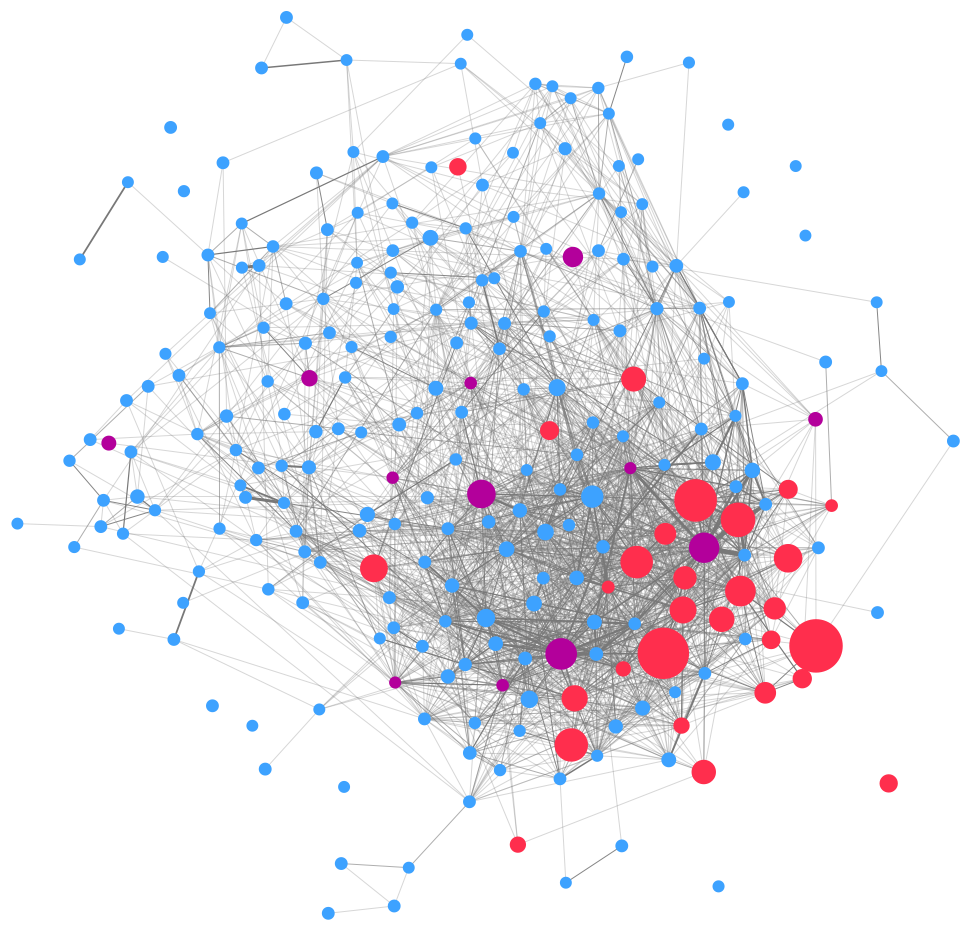
\includegraphics[scale=0.38]{imgs/Institutions.png}
\end{center}
\caption[Firm projection of the directorate network in New York City, 1902]{Firm projection of the directorate network in New York City, 1902. Blue nodes represent financial institutions, red nodes represent railways, and purple nodes represent insurance companies. The size of each node refers to its book value.}
\label{1902firms}
\end{figure}

The average membership in each aspect is calculated. For the financial industry the average membership is $17.21$, for the railroad industry the average membership is $12.76$, and the average membership for insurance companies is $26.17$. Therefore we note that railroads have, on average, lower number of directors and therefore a larger dependence on the directors that they have. Indeed, on average, a director of a railroad company will have a higher influence than a similar director of either a bank or an insurance company \emph{ceteris paribus}.

\paragraph{Aspectual distance.}

The distance of a pair of aspects measures their relatedness in terms of the number of connections that are similar in both aspects as a proportion of all connections in both aspects. During this time in America there existed no institutions regulating the formation of the directorate network. Given this free-market nature, one would expect that intertwining between aspects of the directorate network be reflective of complementarities between industries. Indeed, directors can attain a relatively large payoff from directly operating in industries that are have complementarities.

The distance between each pair of aspects was calculated. The distance from the banking industry to the railroad industry is given as $0.0127$ and $0.0249$ vice versa. The distance from the banking industry to the insurance industry is given as $0.0298$ and $0.0437$ vice versa. Finally, the distance from the railroad industry to the insurance industry is given as $0.0201$ and $0.0221$ vice versa.

\subsection{Centrality of directors and firms}

Microscopic network analysis focuses on the centrality of nodes. Of particular interest is the $\beta$-measure and standard degree measures, as discussed above. We provide an overview of the centrality of individual firms and directors.

\paragraph{$\beta$-measure of directors.}

With the original beta measure a number of directors are indicated as important, these include James Stillman ($1.436$), Edward H. Harriman ($0.988$) George F. Baker ($0.969$), Charles W. Morse ($0.8759$), and William Rockefeller ($0.861$).

It is undeniable that the men highlighted by the $\beta$-measure were highly influential during this time. On James Stillman's death in 1918 he was regarded as one of the wealthiest men in America, with an estimated fortune of \$100,000,000. Although closely tied to the activities of other influential financiers and industrialists such as J.P. Morgan, Edward H. Harriman, and William Rockefeller, his activities were never the subject of public discussion (New York Times, 1918). Between 1902 and the time of Edward H. Harriman's death in 1909 he remained President of the Union Pacific and the Southern Pacific railroad companies, and further controlled the Saint Joseph and Grand Island railway, the Illinois Central railroad, the Central of Georgia railroad, the Pacific Steamship Company, and the Wells Fargo Express Company. Indeed, all directors that have high beta are known to have some financial, speculative, and industrial influence in the early 20th Century. Also, during the beginning of the 20th Century Charles W. Morse organised the so-called \emph{Ice Trust} and made a move to banking, later being affiliated with F. Augustus Heinze during the Panic of 1907. William Rockefeller, brother of J.D. Rockefeller, was a prominent figure in finance, railways, and oil.

\paragraph{$\beta$-measure of firms.}

When aggregating the beta scores of all directors of each firm a number emerge as prominent. Specifically the American Surety Company ($4.21$), the Equitable Life Insurance Society ($3.157$), the Hanover National Bank ($3.111$) the Knickerbocker Trust Company ($2.868$), and the United States Trust Company ($2.623$). The measure of an affiliations beta in this circumstance provides an indication of the number of firms it influences beyond itself. All firms with a high beta are known to be large, however using this method there is little sign of J.P. Morgan and Company.

Importantly there is also little sign of railroad companies when using the original beta measure. Indeed, despite their size and value, railroad companies tended to have fewer directors on average compared to insurance companies and trusts. The original beta measure has an inherent bias toward firms with a large number of directors who themselves are members of other directorates that have a low number of directors. This bias is partially handled with the augmented measure of influence provided in Section~\ref{Theory:Influence}, which takes into consideration the value of firms. Furthermore, the original beta does not consider a multidimensional network.

% Standard degree measure...??

\subsection{Influence and elites in New York City}

Sections~\ref{Theory:Influence} and~\ref{Theory:Elites} introduced a number of tools to assess power and influence in a bipartite network, including the $\sigma$-score and elites. These are applied to the directorate network and the results are assessed below.

\subsubsection*{Firm value and influence}

With respect to the $\beta$-measure, we assumed that the value of all firms is equal to $1$. This assumption is dropped as we now note that the value of some firm $H \in \Gamma$ is equal to $\nu_{H}$. The use of a firms value with regards the $\sigma$-score diminishes the problem of the $\beta$-measure of over-biasing directors who are present on the boards of many small firms, or alternatively under-biasing firms that have a low number of directors but are also on the board of large and high valued firms.

\paragraph{Firm data.}

There are a number of ways to measure the \emph{value} of a firm. Here, we suggest that a firms' value is measured in terms of the book value of its resources. Data was collected from multiple sources. Specifically, data on the asset value of New York City trusts companies, safe deposit companies, and savings banks were gathered from the \emph{Reports of the Superintendent of Banks}, data on National Banks operating in New York were gathered from the \emph{Annual Reports of the Comptroller of the Currency to the Congress of the United States}, which were also published for each year of the analysis. Furthermore, data on the condition of commercial banks operating in New York was compiled by the New York Clearing House and published by the \emph{New York Times}\footnote{The New York Times have published their entire archive of newspapers since 1851 online.} alongside the publication of the Reports of the Superintendent of Banks. Data on the book value of insurance companies was gathered from the \emph{Annual Report of the Superintendent of Insurance to the New York Legislature}. More information regarding the sources can be seen in Table~\ref{vardesc}.

Each of these reports records the balance sheets of individual financial institutions. Specifically, the figures for the book value of resources and liabilities are provided and compartmentalised into separate types of assets and liabilities depending on the type of resources and liabilities in each banks balance sheet. Due to the fact that total resources and total liabilities are recorded for all financial institutions these values are used as the value of each firm.

Alternatively the Market Capitalisation of each firm could be used derived from the share value and number of shares outstanding in each company; however there are three main issues with using this data: (1) The majority of all recorded financial institutions were not publicly floated on the stock market, and therefore the share price and market capitalisation of these institutions are unknown; (2) Out of the financial institutions that were floated the information regarding the number of shares outstanding is still only partial; and (3) The reports published regarding the financial institutions adjusted the book value of their assets and liabilities such that they would better reflect their market values.

\paragraph{Influence of directors.}

The (weighted) $\sigma$-score measures the influence of directors in terms of dollar amounts\footnote{Note that these are non-normalised weighted $\sigma$-scores.}. Specifically, the influence of a director will be proportional to the value of all firms that they are a member of and the number of directors of each firm. When running the measurement, the directors with the highest influence include James Stillman ($222,163,741.5$), Edward H. Harriman ($221,102,348.2$), Hamilton Twombly ($167,033,722.2$), James J. Hill ($161,756,194.5$), and Samuel Rea ($141,321,877.5$).

Although Stillman and Harriman were notable with the beta measure, the introduction of Twombly, Hill, and Rea suggests the removal of bias against directors of railroads which were valued highly, but had a relatively low number of directors. Indeed, Hill was the CEO of Great Northern Railway during this time. Twombly was financial advisor to William Vanderbilt, and made a career in the railroad industry.

\paragraph{Influence of firms.}

The influence of each firm will be given by the $\sigma$-score calculated from the directorate hypergraph. The top firms that emerge from this analysis are the Equitable Life Assurance Society ($1,698,309,975$), the Southern Pacific Company ($1,385,947,753$), the Union Pacific Railroad Company ($1,364,554,939$), the Northern Pacific Railway Company ($1,385,947,753$), and Baltimore and Ohio Railroad Company ($1,301,836,214$).

The Equitable Life Assurance Society remains consistently high in the ranking. However, many of the top firms are railroad companies, which suggests that, despite having a relatively low number of directors, the directors are also directors in other highly valued companies such as other railways and highly valued banks.

\subsubsection*{The elites of New York City}

Elites refer to nodes that exist in all aspects of an aspectual hypergraph. With respect to a directorate network, an elite refers to an agent that is a director of a set of firms such that all firms collectively operate in all industries. An elite network refers to the subsequent network that results from parsing out the elite. Further analysis can be done with respect to the resulting elite structure; indeed, some elites may be more important than others. This can be measured with respect to known centrality measures.

\begin{figure}[t]
\begin{center}
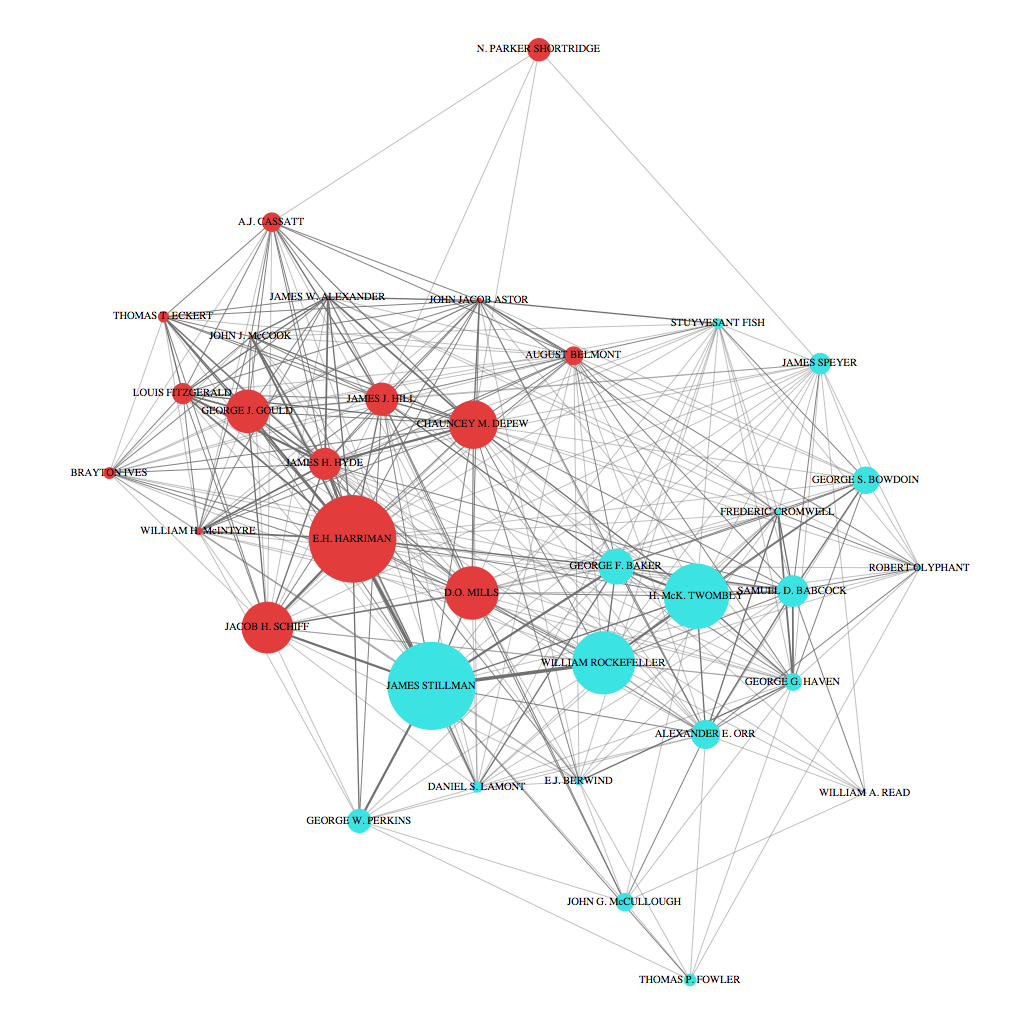
\includegraphics[scale=0.38]{imgs/Elite.png}
\end{center}
\caption[Elite directors in New York City, 1902]{Elite directors in New York City. The larger the node the greater the directors influence. The colour of the node represents the community it is a member of according to Newman's Q.}
\label{Fig:elite}
\end{figure}

The elite structure that emerges can be seen in Figure~\ref{Fig:elite}. There are a number of comments to be made. First, it is notable that from the initial network of $3006$ directors, only $35$ directors remain as elite. Second, the network much more dense with a density of $0.555$. There exists two tightly-knit cores resulting in two distinct communities when using Newman's Q-measure of modularity (Newman, 2006), which subsequently provides a value of $0.224$ for the entire network. These communities are highlighted in red and blue. Third, the diameter of the network is $3$, with an effective diameter of $2$, suggesting that any elite director can contact any other through a single intermediary\footnote{The notion of an effective diameter refers to the lowest resulting diameter after $10\%$ of the nodes in the network have been removed, and was initially proposed by Leskovec et al. (2005). When N. Parker Shortridge, William A. Read, and Thomas P. Fowler are removed from the elite network the diameter drops to 2.}. Finally, the average degree in the network is $18.857$, suggesting that on average each node is connected to over half the network, and the average weighted degree is $33.943$. The degree distribution is relatively normally distributed, with most directors having a degree between $16$ and $19$.

The emergence of elites and the resulting topology of the elite structure is notable due to its non-random nature. Indeed, although $99\%$ of the nodes and links have been removed from the director projection of the bipartite network the elite network that remains is both a single component and substantially more densely connected than the director projection of the bipartite network. This non-random nature indicates that there must exist some strategic network formation; specifically, there is utility to be gained from elites directly connecting to other elites. This could be in the form of both informational benefits and in the form of coordination benefits. Specifically, in this case, elites have direct access to information regarding the operations and the health of all industries and can therefore coordinate activities---such as investment, insurance, and funding---between and within industries.

As predicted, the elite directors have a high propensity to be influential. Specifically, eight out of the top ten most influential directors are elite and fourteen out of the top twenty-five are elite. Those directors who have a higher influence have a greater propensity to be more central in the elite structure when considering conventional centrality measures, whilst those directors with little influence are more peripheral.

The most central members of the elite also constitute a substantial number of the National Securities Company's members. Specifically, Stillman, Harriman, Schiff, Lamont, Baker, Hill, and Perkins were directors in the National Securities Company; and all play significantly central roles in the network. Even when removing the National Securities Company from the network and recalculating the elite, all directors remain notably central. This suggests, from purely case-study evidence, that elites were not only important for influence, but also control between industries.

\paragraph{Power and control in the elite.}

We look at measures of centrality for the elite network. There are a number of off-the-shelf measures to calculate the centrality of nodes within an undirected network. We also noted some measures, such as brokerage and criticality, which are specifically created to measure the power of individual nodes (brokerage) and sets of nodes (criticality).

We first look at off-the-shelf measures of centrality. Table~\ref{CentralElite} provides the centrality statistics for the 10 most central directors in the Elite structure. We note that although different centrality measures provide a slightly different ranking order than other centrality measures, there tends to be some consistency regarding the importance of Edward H. Harriman, James Stillman, Darius O. Mills, Chauncey M. Depew, and James J. Hill.

\begin{table}[t]
\resizebox{\textwidth}{!}{%
\centering
\begin{tabular}{ l c c c c c c} \hline
Director	           & $\delta_{i}$ 	& Weighted $\delta_{i}$ & Closeness   & Betweenness  & Eigenvector & Criticality \\ \hline
Edward H. Harriman	   &	$28$	&	$74$	       &	$0.850$	 &	$0.025$	    &	$0.997$	&	$0.401$\\
James H. Hyde	       &	$25$	&	$64$	       &	$0.790$	 &	$0.022$	    &	$0.898$	&	$0.364$\\
James Stillman	       &	$24$	&	$62$	       &	$0.772$	 &	$0.037$	&	$0.801$	&	$0.352$\\
Chauncey M. Depew	   &	$29$	&	$58$	       &	$0.871$	 &	$0.044$	&	$0.999$	&	$0.414$\\
George F. Baker	       &	$23$	&	$46$	       &	$0.755$	 &	$0.020$	&	$0.796$	&	$0.341$\\
James J. Hill	       &	$24$	&	$45$	       &	$0.772$	 &	$0.033$	&	$0.832$	&	$0.353$\\
Darius O. Mills	       &	$29$	&	$44$	       &	$0.871$	 &	$0.040$	&	$1.000$	&	$0.411$\\
John Jacob Astor	   &	$23$	&	$44$	       &	$0.755$	 &	$0.016$	&	$0.837$	&	$0.339$\\
Henry Twobley	       &	$19$	&	$43$	       &	$0.693$	 &	$0.009$	&	$0.677$	&	$0.288$\\
Jacob H. Schiff	       &	$24$	&	$41$	       &	$0.772$	 &	$0.016$	&	$0.870$	&	$0.340$\\ \hline
\end{tabular}
}
\caption{Centrality statistics of 10 most central directors in the elite structure.}
\label{CentralElite}
\end{table}

Due to the well-connected nature of the elite structure there are no middlemen and therefore no opportunity for brokerage. However, the incomplete nature of the network allows for the existence of blocks. When the criticality measure is applied the the elite structure we find that are the most important. Note that all but one of these individuals exist in the Northern Securities Company; indeed, it is acceptable to conclude that these directors could collectively control and manipulate main trusted channels of information between all industries of the economy.

\section{Economic performance and centrality} \label{Application:Regression}

Thus far we have developed tools to measure influence and elites and applied these to the directorate network of New York City. It was noted through the anecdotal evidence of the Northern Securities Company that elites have significant power in multiple industries of the economy, and that highly influential firms, i.e., firms with a large $\sigma$-score, were economically dominant. Here we assess whether these are general phenomena and thus answer the initial research question of whether the influence of a firms' directorate has an impact on its economic performance.

Of specific interest is the ability for a financial institution to generate profit and increase its size as a consequence of the centrality of a firms' directorate. As hypothesised above, the size and influence of the firms' directorate network should have an impact on the performance and profitability of the firm. This relationship may emerge from a number of sources, for example, from the ability for firms to borrow funds from other financial institutions to invest in entrepreneurial opportunities. Indeed, we would expect that a more connected financial institution would be able to exploit social relations, indicated by overlapping portfolios, and therefore reduce any uncertainty in the loan and investment opportunity. Although data from insurance, railroads, and banking are gathered the specific interest of this research is in financial institutions only.

\subsection{Overview of data}

The data gathered and analysed can be partitioned into two types: the first is the network data, and the second is balance-sheet data. The source of the network data has been discussed above; all centrality measures, apart from influence and external influence, were calculated from this data. This centrality data is complete for all firms and financial institutions. Balance-sheet data was acquired from multiple sources as discussed before. Data on the value of all financial institutions resources was attained, however data on the full balance sheet of each financial institution is incomplete.

\subsubsection*{Variable descriptions}

Descriptions of all variables used in the regression analysis are provided in Table~\ref{vardesc}. This table includes all relevant balance sheet data used in the analysis as well as dummy variables. There are two sets of dummy variables, the first set relates to the type of financial institution which includes State banks, National banks, Savings bank, and a Trust, and the second set relates to the location of the headquarters of the financial institution in either one of five boroughs of New York City, either Manhattan, Brooklyn, Queens, the Bronx, or Staten Island.

\begin{table}[t!]
\resizebox{\textwidth}{!}{%
\begin{tabular}{lll} \hline
{\bf Variable name}         & {\bf Description}                                                                                                                                                                    & {\bf Source} \\ \hline
Profits ($\pi_{i}$)               & Profits made by firm as indicated on January 1st 1903. & \emph{b,c,d}        \\
Size ($\nu_{i}$)                  & Size of the firm measured by the book value of the firms total assets.                                                                                                                                                             & \emph{b,c,d}        \\
\begin{tabular}[c]{@{}l@{}}Interbank\\ Borrowing\end{tabular}  & \begin{tabular}[c]{@{}l@{}}Total amount of money due to all other financial institutions in January\\ 1st 1903. This includes all money lent out to trust companies, savings banks,\\ State banks and National banks.\end{tabular} & \emph{b,c,d}        \\
Liquid                & \begin{tabular}[c]{@{}l@{}}Total amount of cash on hand. This includes all liquid assets such as specie,\\ banknotes, checks, and other cash items.\end{tabular}                                                                    & \emph{b,c,d}        \\
Illiquid              & Total amount of money held in the form of stocks, bonds, and mortgages.                                                                                                                                                             & \emph{b,c,d}        \\
\begin{tabular}[c]{@{}l@{}}Interbank\\ Lending\end{tabular} & \begin{tabular}[c]{@{}l@{}}Total amount of money lent out to all other banks including Savings banks,\\ State banks, National banks, and trust companies. Amounts recorded in \\ January 1st 1903.\end{tabular}                    & \emph{b,c,d}        \\
Year                  & The number of years that the firm has been operating.                                                                                                                                                                              & \emph{a}            \\
Directors             & Number of directors in the firm in September 1902.                                                                                                                                                                                 & \emph{a}            \\
$\sigma_{i}$              & The influence of a firm given by its $\sigma$-score.                                                                                                                                                                               & \emph{a,b,c,d,e}            \\
$\sigma^{\star}_{i}$                 & The external influence of a fir.                                                                                                                                                                                                  & \emph{a,b,c,d,e}            \\
Elites                & The number of elite directors in the firm.                                                                                                                                                                                         & \emph{a,e}            \\
$\beta^{\star}_{i}$   & The generalised $\beta$-measure of a firm in the affiliation projection.                                                                                                                                                                       & \emph{a,e}            \\
Criticality           & The criticality score of a firm in the affiliation projection.                                                                                                                                                                     & \emph{a,e}            \\
$\delta_{i}$          & \begin{tabular}[c]{@{}l@{}}The degree of the firm in the affiliation projection. The total number of \\ other firms that the firm has direct interlocks with.\end{tabular}                                                         & \emph{a, e}            \\
Weighted $\delta_{i}$ & The sum of all weighted interlocks with other firms in the affiliation network.                                                                                                                                                    & \emph{a,e}            \\
Cluster               & The local clustering coefficient of the firm in the affiliation projection.                                                                                                                                                        & \emph{a,e}            \\
PageRank              & The PageRank centrality of the firm in the affiliation projection.                                                                                                                                                                 & \emph{a,e}            \\
Closeness             & The normalised closeness centrality of the firm in the affiliation projection.                                                                                                                                                     & \emph{a,e}            \\
Betweenness           & The normalised betweenness centrality of the firm in the affiliation projection.                                                                                                                                                   & \emph{a,e}            \\
Eigenvector           & The weighted eigenvector centrality of the firm in the affiliation projection.                                                                                                                                                     & \emph{a,e}            \\
StateDum              & Dummy variable. Equal to $1$ if firm is a State Bank and $0$ otherwise.                                                                                                                                                                 & \emph{b,c,d}        \\
NatDum                & Dummy variable. Equal to $1$ if firm is a National Bank and $0$ otherwise.                                                                                                                                                            & \emph{b,c,d}        \\
SavingsDum            & Dummy variable. Equal to $1$ if firm is a Savings Bank and $0$ otherwise.                                                                                                                                                               & \emph{b,c,d}        \\
TrustDum              & Dummy variable. Equal to $1$ if firm is a Trust and $0$ otherwise.                                                                                                                                                                    & \emph{b,c,d}        \\
BronxDum              & Dummy variable. Equal to $1$ if firm is situated in the Bronx and $0$ otherwise.                                                                                                                                                      & \emph{a}            \\
BrookDum             & Dummy variable. Equal to $1$ if firm is situated in Brooklyn and $0$ otherwise.                                                                                                                                                       & \emph{a}            \\
ManhatDum             & Dummy variable. Equal to $1$ if firm is situated in Manhattan and $0$ otherwise.                                                                                                                                                      & \emph{a}            \\
QueensDum             & Dummy variable. Equal to $1$ if firm is situated in Queen's and $0$ otherwise.                                                                                                                                                        & \emph{a}            \\
StatenDum             & Dummy variable. Equal to $1$ if firm is situated in Staten Island and $0$ otherwise.                                                                                                                                                  & \emph{a}  \\ \hline
\end{tabular}
}
\begin{flushleft}
\emph{Note: `a' refers to the Directory of Directors of New York City, `b' refers to the Annual Report of the Superintendent of Banks 1903, `c' refers to the Annual Report of the Comptroller of the Currency 1902, `d' refers to the New York Times, and `e' refers to calculation.}
\end{flushleft}
\caption{Description of variables used for regression analysis}
\label{vardesc}
\end{table}

Data from bank balance sheets was analysed. Of specific interest was the total value of all liquid assets, such as specie, banknotes and other cash items, and illiquid assets, in the form of securities. So too were the financial institutions' interbank borrowing and lending characteristics.

A notable omission from the data is a measure of Tobin's Q, due to the inability to attain full stock market data of all institutions during this time. Other notable papers use Tobin's Q as an indicator to the health and economic performance of the firm. Indeed, future research regarding the relationship between directorate centrality and firm performance should take advantage of stock market data and derived measures such as Tobin's Q.

\subsubsection*{Data summary statistics}

The summary statistics of all variables used can be seen in Table~\ref{fin-ss} in Appendix~\ref{B}. The full network of financial institutions includes $63$ State banks, $49$ National banks, $51$ Savings banks, and $47$ trusts. Despite there being fewer trusts, they are more substantially connected than any other type of firm, including railroads and insurance companies. Indeed, firms are connected to $4.35$ different trusts on average, compared to $3.13$ National banks, $2.44$ State banks, and $1.7$ Savings banks.

On average financial institutions are connected to $15.51$ other firms through an overlapping directorate, however, much like other social and natural systems, the degree distribution is non-normal. Specifically, the frequency of nodes' degrees follows a distribution more akin to a power-law. Subsequently, most of the centrality measures, which are derived from the structure of the directorate hypergraph and affiliation projection, follow the same power-law distribution. All centrality measures have a skewed distribution suggesting that many firms have a low centrality, with a few having a relatively high centrality. Closeness centrality nor the $\beta$-measure follow the same power-law distributions as the other centrality measures. Closeness centrality is reflective of the density and average path length in the network, thus, with a well-connected network, many of the closeness centralities of individual firms are similar and converge to $1$ as the network densifies. The distribution of the $\beta$-measure has a negative kurtosis.

Data on the size and centrality of financial institutions is complete. However, balance sheet data was incomplete especially with respect to the interbank borrowing of savings banks.

\paragraph{Correlation matrix.}

The matrix in Table~\ref{fin-corr} shows dependence relationships of variables in the form of Pearson correlation coefficients between all pairs of financial data variables and important centrality measures used throughout the analysis.

A number of points are notable here. First, there exists only a weak positive correlation between the interbank borrowing and interbank lending of a financial firm, suggesting a a potential imbalance between the amount an institution borrows and the amount it lends, which implies the existence of surplus and deficit institutions. Second, there exists a high correlation between the size of a firm (the value of its total assets) and the interbank borrowing, the amount of liquid and illiquid assets of the firm. The inclusion of size and interbank borrowing, or any pairs of highly correlated variables, may bias the analysis. Third, all centrality measures are very highly correlated with each other. Again, the inclusion of all highly correlated centrality measures can bias the coefficients of the regression. Fourth, there exists high correlation between the size of the firm and all centrality measures. Finally, the relationship between the number of directors and profit is relatively low.

\begin{table}[t!]
\begin{onehalfspace}
\centering
\resizebox{\textwidth}{!}{%
\begin{tabular}{@{\extracolsep{5pt}} lcccccccccccccc}
\\[-1.8ex]\hline
\hline \\[-1.8ex]
                                                              & \begin{tabular}[c]{@{}c@{}}Profit\\($\pi_{i}$)\end{tabular} & \begin{tabular}[c]{@{}c@{}}Interbank\\borrowing\end{tabular} & Liquid & Illiquid & \begin{tabular}[c]{@{}c@{}}Interbank\\lending\end{tabular} & Years  & Directors & \begin{tabular}[c]{@{}c@{}}Size\\($\nu_{i}$)\end{tabular} & $\sigma_{i}$ & Elite & $\delta_{i}$ & \begin{tabular}[c]{@{}c@{}}Weighted\\ $\delta_{i}$\end{tabular} & Eigenvector & $\beta^{\star}_{i}$ \\ \hline
Profit ($\pi_{i}$)                                                        & 1.000  &                                                               &        &          &                                                             &        &           &       &              &       &              &                                                                 &             &             \\
\begin{tabular}[c]{@{}l@{}}Interbank\\ borrowing\end{tabular} & 0.181  & 1.000                                                         &        &          &                                                             &        &           &       &              &       &              &                                                                 &             &             \\
Liquid                                                        & 0.283  & 0.861                                                         & 1.000  &          &                                                             &        &           &       &              &       &              &                                                                 &             &             \\
Illiquid                                                      & 0.131  & 0.586                                                         & 0.113  & 1.000    &                                                             &        &           &       &              &       &              &                                                                 &             &             \\
\begin{tabular}[c]{@{}l@{}}Interbank\\ lending\end{tabular}   & 0.091  & 0.340                                                         & 0.200  & 0.342    & 1.000                                                       &        &           &       &              &       &              &                                                                 &             &             \\
Years                                                         & 0.142  & 0.321                                                         & 0.338  & 0.387    & 0.125                                                       & 1.000  &           &       &              &       &              &                                                                 &             &             \\
Directors                                                     & 0.045  & 0.028                                                         & -0.118 & 0.461    & 0.462                                                       & -0.091 & 1.000     &       &              &       &              &                                                                 &             &             \\
Size ($\nu_{i}$)                                                & 0.325  & 0.829                                                         & 0.708  & 0.600    & 0.384                                                       & 0.370  & 0.220     & 1.000 &              &       &              &                                                                 &             &             \\
$\sigma_{i}$                                                      & 0.185  & 0.391                                                         & 0.410  & 0.229    & 0.329                                                       & 0.087  & 0.298     & 0.612 & 1.000        &       &              &                                                                 &             &             \\
Elite                                                         & 0.108  & 0.260                                                         & 0.265  & 0.103    & 0.221                                                       & -0.014 & 0.276     & 0.441 & 0.902        & 1.000 &              &                                                                 &             &             \\
$\delta_{i}$                                                  & 0.168  & 0.320                                                         & 0.318  & 0.253    & 0.330                                                       & 0.048  & 0.352     & 0.535 & 0.860        & 0.789 & 1.000        &                                                                 &             &             \\
Weighted $\delta_{i}$                                         & 0.177  & 0.323                                                         & 0.327  & 0.237    & 0.314                                                       & 0.042  & 0.362     & 0.556 & 0.917        & 0.875 & 0.968        & 1.000                                                           &             &             \\
Eigenvector                                                   & 0.179  & 0.339                                                         & 0.354  & 0.231    & 0.298                                                       & 0.102  & 0.275     & 0.536 & 0.885        & 0.814 & 0.967        & 0.948                                                           & 1.000       &             \\
$\beta^{\star}_{i}$                                                   & 0.173  & 0.235                                                         & 0.188  & 0.211    & 0.260                                                       & -0.078 & 0.421     & 0.404 & 0.558        & 0.503 & 0.729        & 0.712                                                           & 0.592       & 1.000       \\
\hline \\[-1.8ex]
\end{tabular}
}
\caption{Correlation matrix of financial data and network centralities.}
\label{fin-corr}
\end{onehalfspace}
\end{table}


The assessment of the correlation matrix suggests that the $\sigma$-score, weighted degree, and eigenvector centralities should be most relevant in explaining the relationship between directorate centrality and economic performance. This is indeed highlighted with the regression analysis.

\subsection{Comparing financial institutions, insurance companies and railroads}

Before the regression analysis we provide a comparison of financial institutions, insurance companies, and railroads, noting fundamental differences between them. Figure~\ref{firm-type1} highlights differences in the variance between the size of the firms, the number of directors in the firm, and its influence. Notably, we find that the variance of the number of directors and value of banks is low relative to insurance companies and railroads. Insurance companies have a relatively high variance in the number of directors and railroads have a relatively high variance in the value of its assets.

\begin{figure}[t]
\label{firm-type1}
\centering
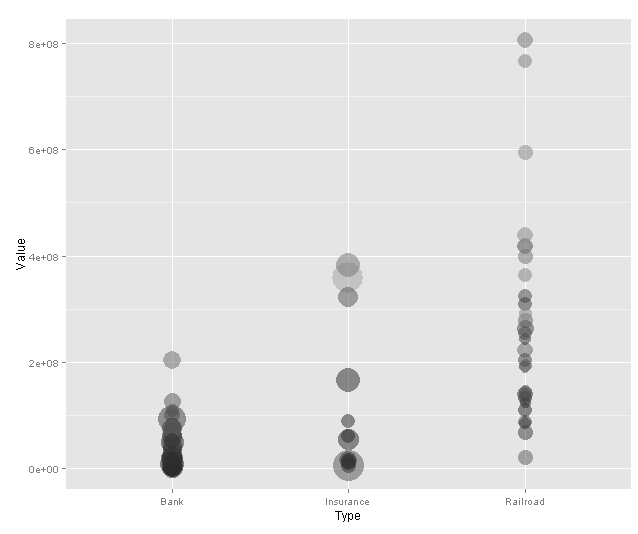
\includegraphics[width=0.7\textwidth]{imgs/firm-type2.png}
\caption{Distribution of firm value per industry}
\end{figure}

This assessment highlights that different types of firm can have substantially different fundamental characteristics. Notably, as is found below, the type of directorial overlap may matter more than the number of directorial overlaps.

\subsection{Regression analysis}

We use OLS regressions to assess the relationship between the centrality of the firm and the profits generated by it. A number of relationships are assessed; the first looks at the profits generated by the financial institutions and the centrality of the institutions' directorate, and the second investigates the size or value of the financial institutions assets and the centrality of the institution.

\subsubsection*{Profit and centrality}

The Regression model in Equation~\ref{eq:regprofit} is used to derive the relationship between a firms' directorate centrality and its profitability. Multiple centrality measures are used independent of each other and, as a consequence, we allow $Centrality_{i}$ to denote a form of centrality used in the specific regression. The centrality measures used in this analysis include the $\sigma$-score and number of Elites from the directorate hypergraph, the degree of the firm ($\delta$), eigenvector, $\beta$-measure and weighted degree from the affiliation projection. As a consequence, multiple regressions are used to find the relationship between profit and individual centrality measures. The regression equation is given by:

\begin{multline} \label{eq:regprofit}
\pi_{i} = b_{0} + b_{1}~Liquid_{i} + b_{2}~Illiquid_{i} + b_{3}~IBLending_{i} + b_{4}~Years^{2}_{i}\\
+ b_{5}~Directors_{i} + b_{6}~Centrality_{i} + \epsilon_{i}
\end{multline}
where $b_{v}$ is the co-efficient of the corresponding $v^{th}$ explanatory variable and $b_{0}$ is the intercept.

\paragraph{Interpretation of results.}

The result of the regressions can be seen in Table~\ref{regress:profit}. Each OLS regression includes 117 observations where all relevant data on financial institutions is complete. The total value of all liquid assets is quite consistent and highly statistically significant in all regressions regardless of centrality measure used. This suggests that as a firms' liquid assets increase by \$1,000,000 then the firms' profits should increase by approximately \$120,000. Moreover, the square of the number of years in operation is also consistent and statistically significant to 10\% and 5\% levels. This suggests that for every new year a firm is in operation its profit should increase by approximately \$10,000. All other variables, such as the total amount of Interbank lending, the total amount of Illiquid assets, and the number of directors all remain statistically insignificant at 10\% levels.

\begin{table}[t!] \centering
\resizebox{\textwidth}{!}{%
\begin{tabular}{@{\extracolsep{5pt}}lD{.}{.}{-3} D{.}{.}{-3} D{.}{.}{-3} D{.}{.}{-3} D{.}{.}{-3} D{.}{.}{-3} }
\\[-1.8ex]\hline
\hline \\[-1.8ex]
 & \multicolumn{6}{c}{\textit{Dependent variable:}} \\
\cline{2-7}
\\[-1.8ex] & \multicolumn{6}{c}{Profit ($\pi_{i}$)} \\
\\[-1.8ex] & \multicolumn{1}{c}{(1)} & \multicolumn{1}{c}{(2)} & \multicolumn{1}{c}{(3)} & \multicolumn{1}{c}{(4)} & \multicolumn{1}{c}{(5)} & \multicolumn{1}{c}{(6)}\\
\hline \\[-1.8ex]
 Liquid & 0.113^{***} & 0.117^{***} & 0.120^{***} & 0.118^{***} & 0.121^{***} & 0.123^{***} \\
  & (0.015) & (0.015) & (0.015) & (0.015) & (0.016) & (0.016) \\
  Illiquid & 0.002 & 0.004 & 0.008 & 0.005 & 0.008 & 0.010 \\
  & (0.013) & (0.013) & (0.013) & (0.013) & (0.013) & (0.013) \\
  IBLending & 0.043 & 0.042 & 0.040 & 0.044 & 0.037 & 0.037 \\
  & (0.034) & (0.034) & (0.035) & (0.035) & (0.035) & (0.036) \\
  Years$^2$ & 0.0001^{*} & 0.0001^{**} & 0.0001^{**} & 0.0001^{**} & 0.0001^{**} & 0.0001^{**} \\
  & (0.00003) & (0.00003) & (0.00003) & (0.00003) & (0.00003) & (0.00003) \\
  Directors & 0.004 & 0.005 & 0.007 & 0.003 & 0.009 & 0.009 \\
  & (0.013) & (0.013) & (0.013) & (0.013) & (0.013) & (0.015) \\
  $\sigma_{i}$ & 11.234^{***} &  &  &  &  &  \\
  & (3.727) &  &  &  &  &  \\
  $\sigma^{\star}_{i}$ &  & 10.589^{***} &  &  &  &  \\
  &  & (3.882) &  &  &  &  \\
  Elites &  &  & 0.070^{**} &  &  &  \\
  &  &  & (0.032) &  &  &  \\
  Weighted $\delta_{i}$ &  &  &  & 0.006^{**} &  &  \\
  &  &  &  & (0.002) &  &  \\
  $\delta_{i}$ &  &  &  &  & 0.006 &  \\
  &  &  &  &  & (0.004) &  \\
  $\beta^{\star}_{i}$ &  &  &  &  &  & 0.087 \\
  &  &  &  &  &  & (0.105) \\
  Constant & 0.071 & 0.062 & 0.044 & 0.030 & -0.021 & -0.019 \\
  & (0.188) & (0.190) & (0.191) & (0.189) & (0.191) & (0.193) \\
 \hline \\[-1.8ex]
Observations & \multicolumn{1}{c}{117} & \multicolumn{1}{c}{117} & \multicolumn{1}{c}{117} & \multicolumn{1}{c}{117} & \multicolumn{1}{c}{117} & \multicolumn{1}{c}{117} \\
R$^{2}$ & \multicolumn{1}{c}{0.625} & \multicolumn{1}{c}{0.620} & \multicolumn{1}{c}{0.612} & \multicolumn{1}{c}{0.615} & \multicolumn{1}{c}{0.602} & \multicolumn{1}{c}{0.597} \\
Adjusted R$^{2}$ & \multicolumn{1}{c}{0.605} & \multicolumn{1}{c}{0.599} & \multicolumn{1}{c}{0.591} & \multicolumn{1}{c}{0.594} & \multicolumn{1}{c}{0.580} & \multicolumn{1}{c}{0.575} \\
\hline
\hline \\[-1.8ex]
\textit{Note:}  & \multicolumn{6}{r}{$^{*}$p$<$0.1; $^{**}$p$<$0.05; $^{***}$p$<$0.01} \\
\end{tabular}
}
\caption{Results of profit-centrality regressions}
\label{regress:profit}
\end{table}

A number of centrality measures are tested, which include the $\sigma$-score of the financial institution, the number of elite directors in the institution, the degree and weighted degree of the institution, the institutions eigenvector and its $\beta$-measure. The $\sigma$-score has a positive, statistically significant relationship with the firms profit at a 99\% level, suggesting that as a firms influence increases by \$1,000,000 then its profit should increase by \$86,900. The number of elites has a positive, statistically significant relationship with the firms profit at a 95\% level, suggesting that as a firm increases the number of elites in its board by 1 it will lead to a generation of profits by \$70,000. Also, the weighted degree of a firm in the affiliation projection has a positive, statistically significant relationship with the firms profit at a 90\% level. This relationship suggests that if any one of a firms directors increases the number of boards that they are on by 1 then this will lead to an increase in profits by \$6,000.

Other recorded centrality measures, such as the degree of the firm, it's eigenvector centrality, and it's $\beta$-measure are all positively related to the firms profit, but none of which are statistically significant at a 90\% level. The insignificance of degree centrality suggests that the total number of overlapping directorates a firm has does not have an impact on its economic performance. Indeed, the number of links of the firm in the affiliation projection is not important to its profitability; rather the weight and the context of the links are more influential. Note that all other centrality measures, such as betweenness, closeness, PageRank, and the firms local clustering co-efficient were all tested but none of which are statistically significant to a 90\% level.

\paragraph{Location and firm-type dummies.}

The data consists of different types of financial institution, including National banks, State banks, Saving banks, and Trust companies. These financial institutions are located in different boroughs of New York City. Regressions are carried out to test the importance of firm type and location factors, the results of which can be seen in Table~\ref{profit-type-location} in Appendix~\ref{B}. The regression finds that National banks persistently have lower profit levels, suggesting that if a financial institution is a National bank then its profit will be approximately \$480,000 lower than other types of financial institution. All other firm-type and location dummies are recorded as statistically insignificant at the 90\% confidence level.

\paragraph{Interlock types.}

The initial regression showed that, in many cases, the centrality and connectivity of the financial institution was subsequently related to the institutions profits. We disaggregate the interlocks of each institution by counting the number of National banks, State banks, Savings banks, Trust companies, Insurance companies and Railroads each firm has an interlock with and perform a corresponding regression. The results can be seen in Table~\ref{profit-interlock-type} in Appendix~\ref{B}. We find that there is a positive, statistically significant relationship between the number of railroads a financial institution has an interlock with and the profitability of the financial institution. Specifically, we find that if a financial institution forms a new interlock with a railroad then this will generate an increase in profits of \$48,000. All other types of interlock are not found to be statistically significant at a 90\% level. This partitioning of a firms link set into firm types provides a deeper insight into the connectivity of the firm and may provide some explanation as to the inefficacy of the degree centrality to explain the profitability of the firm. Indeed, it may not be so simple as to suggest that the number of firms a financial institution is linked to is important; rather it can be seen that the type of firm a financial institution is connected to is also important. Such a concept is contained in the $\sigma$-score and $\sigma^{\star}$-score since, as noted above, railroads have a high value relative to other financial institutions and insurance companies.

Conversely, if a financial institution were to form an interlocking relation with a national bank then the profits of the firm will decrease by approximately \$60,000. All other types of interlock are not found to be statistically significant at a 90\% level. An explanation can be made for the negative relationship between National bank interlocks and low profit. We find that 13 out of 49 National banks have an above random number of interlocks with other National banks, these 13 firms with above random interlocks with other National banks are disproportionately low profit firms. Specifically, if we rank the set of National Banks in terms of profit we find that 9 out of the 13 National banks with larger than random interlocks are in the lower half of ranking order. Indeed, there exists positive assortative mixing of low profit National banks thus leading to the statistically significant finding.

To conclude, we note that the number of directorial overlaps does not have a statistically significant impact on the profitability of the financial institution. However, the type and context of the overlapping directorates matters for profitability, and this is not included in degree, eigenvector, beta, betweenness, or closeness centrality measures. We find that if firms are connected to more railroads then it will translate to a statistically significant increase in its profitability; firm type is captured in some way by nodal influence ($\sigma$) and external influence ($\sigma^{\star}$), therefore these centrality measure have statistically significant explanatory power.

\subsubsection*{Size and centrality}

Much like above we assess the relationship between the size of the financial institution in terms of the total value of its assets and its centrality, given by a number of different measures including the $\sigma$-score and number of elites. We follow much the same structure as the regression model in equation~\ref{eq:regprofit}, however we include interbank lending in this analysis. The resulting regression equation can be seen in Equation~\ref{eq:regsize} below:
\begin{multline} \label{eq:regsize}
\nu_{i} = \gamma_{0} + \gamma_{1}~Liquid_{i} + \gamma_{2}~Illiquid_{i} + \gamma_{3}~IBBorrowing_{i} + \gamma_{4}~IBLending_{i}\\
+ \gamma_{5}~Years^{2}_{i} + \gamma_{6}~Directors_{i} + \gamma_{7}~Centrality_{i} + \mu_{i}
\end{multline}
where $\gamma_{v}$ is the co-efficient of the corresponding $v^{th}$ explanatory variable and $\gamma_{0}$ is the intercept.

\paragraph{Interpretation of results.}

From the correlation matrix in Table~\ref{fin-corr} we found that the size of a firm was highly correlated with all centrality measures recorded, most specifically with the $\sigma$-score. This high correlation is to be expected since a firms $\sigma$-score is specifically dependent on its own size. The external influence of a firm, given by the $\sigma^{\star}$-measure is not dependent on the firms' own size, but the size of the firms that it has an overlapping directorate with.

The regression results can be seen in Table~\ref{reg:size}. With consideration to the non-centrality measures we find that the total amount of liquid assets, the total amount of illiquid assets, and the total amount of the financial institutions interbank borrowing is positively and significantly related to its value. This suggests that a firm that borrows more will have a higher value, which implies that firms of a larger size has an ability to borrow more. These results are robust across all centrality measures considered. Conversely, Interbank lending is inversely related to firm size, which is consistently significant to a 90\% confidence level in 4 out of 6 regression.

With regards to the centrality measures we find, unsurprisingly, that all measures are positively and significantly related to the size of the firm at 99\% levels and all generate an R$^2$ of over 0.8. When comparing centrality measures we find that the $\sigma$-score has the most explanatory power relative to the others. The weighted degree of a firm also has strong explanatory power, suggesting that if any one of a firms directors were to increase the number of directorates they participated in by 1 then this would lead to an increase of a firms size by \$279,000. Likewise, if a firm increased the number of elites in its directorate by 1 then this would be reflected in an increase in the size of the firm by \$2,977,000. Further, if a firms beta were to increase by 1 then this would lead to an increase in the size of the firm by \$7,160,000.

Other centrality measures---such as betweenness, eigenvector, and PageRank---are also statistically significant at a 99\% level. However, the local clustering co-efficient and closeness remain insignificant at a 90\% level.

\begin{table}[t] \centering
\resizebox{\textwidth}{!}{%
\begin{tabular}{@{\extracolsep{5pt}}lD{.}{.}{-3} D{.}{.}{-3} D{.}{.}{-3} D{.}{.}{-3} D{.}{.}{-3} D{.}{.}{-3} }
\\[-1.8ex]\hline
\hline \\[-1.8ex]
 & \multicolumn{6}{c}{\textit{Dependent variable:}} \\
\cline{2-7}
\\[-1.8ex] & \multicolumn{6}{c}{Size ($\nu_{i}$)} \\
\\[-1.8ex] & \multicolumn{1}{c}{(1)} & \multicolumn{1}{c}{(2)} & \multicolumn{1}{c}{(3)} & \multicolumn{1}{c}{(4)} & \multicolumn{1}{c}{(5)} & \multicolumn{1}{c}{(6)}\\
\hline \\[-1.8ex]
 Liquid & 1.410^{***} & 1.497^{***} & 1.760^{***} & 1.591^{***} & 1.669^{***} & 1.853^{***} \\
  & (0.477) & (0.492) & (0.505) & (0.484) & (0.505) & (0.524) \\
  Illiquid & 0.871^{***} & 0.946^{***} & 1.109^{***} & 0.932^{***} & 0.968^{***} & 1.113^{***} \\
  & (0.245) & (0.252) & (0.255) & (0.248) & (0.261) & (0.267) \\
  IBLending & -1.285^{*} & -1.381^{**} & -1.291^{*} & -1.078 & -1.270^{*} & -1.084 \\
  & (0.668) & (0.690) & (0.717) & (0.688) & (0.716) & (0.765) \\
  IBBorrowing & 1.307^{***} & 1.350^{***} & 1.236^{***} & 1.271^{***} & 1.279^{***} & 1.208^{***} \\
  & (0.237) & (0.245) & (0.253) & (0.242) & (0.252) & (0.264) \\
  Years$^2$ & 0.001 & 0.001 & 0.001^{*} & 0.001 & 0.001 & 0.001^{*} \\
  & (0.0005) & (0.001) & (0.001) & (0.001) & (0.001) & (0.001) \\
  Directors & 0.323 & 0.382 & 0.450^{*} & 0.223 & 0.362 & 0.293 \\
  & (0.238) & (0.245) & (0.253) & (0.251) & (0.258) & (0.290) \\
  $\sigma_{i}$ & 449.234^{***} &  &  &  &  &  \\
  & (69.721) &  &  &  &  &  \\
  $\sigma^{\star}_{i}$ &  & 417.640^{***} &  &  &  &  \\
  &  & (74.488) &  &  &  &  \\
  Elites &  &  & 2.977^{***} &  &  &  \\
  &  &  & (0.633) &  &  &  \\
  Weighted $\delta_{i}$ &  &  &  & 0.279^{***} &  &  \\
  &  &  &  & (0.047) &  &  \\
  $\delta_{i}$ &  &  &  &  & 0.390^{***} &  \\
  &  &  &  &  & (0.082) &  \\
  $\beta^{\star}_{i}$ &  &  &  &  &  & 7.160^{***} \\
  &  &  &  &  &  & (2.050) \\
  Constant & -1.584 & -2.021 & -2.485 & -3.011 & -5.100 & -4.952 \\
  & (3.594) & (3.713) & (3.836) & (3.641) & (3.779) & (3.932) \\
 \hline \\[-1.8ex]
Observations & \multicolumn{1}{c}{124} & \multicolumn{1}{c}{124} & \multicolumn{1}{c}{124} & \multicolumn{1}{c}{124} & \multicolumn{1}{c}{124} & \multicolumn{1}{c}{124} \\
R$^{2}$ & \multicolumn{1}{c}{0.856} & \multicolumn{1}{c}{0.846} & \multicolumn{1}{c}{0.835} & \multicolumn{1}{c}{0.850} & \multicolumn{1}{c}{0.836} & \multicolumn{1}{c}{0.823} \\
Adjusted R$^{2}$ & \multicolumn{1}{c}{0.847} & \multicolumn{1}{c}{0.836} & \multicolumn{1}{c}{0.825} & \multicolumn{1}{c}{0.840} & \multicolumn{1}{c}{0.826} & \multicolumn{1}{c}{0.812} \\
\hline
\hline \\[-1.8ex]
\textit{Note:}  & \multicolumn{6}{r}{$^{*}$p$<$0.1; $^{**}$p$<$0.05; $^{***}$p$<$0.01} \\
\end{tabular}
}
\caption{Results of size-centrality regressions}
\label{reg:size}
\end{table}

\paragraph{Location and firm-type dummies.}

Location and firm-type dummies are added to the regression analysis. As with the regression analysis of profit and centrality above we find that national banks have a persistently low size relative to state banks and trust companies. This persistent negative relationship to a firms size is statistically significant to a 95\% level. Specifically, we find that, when all other factors remain constant, if a financial institution is a national bank then the total value of its asset base will be approximately \$500,000 lower than if it were another type of financial institution. The location dummies are persistently insignificant and the centrality measures remain either statistically significant or insignificant as in Table~\ref{reg:size}.

\paragraph{Interlock types.}

We regress the aforementioned balance-sheet variables with firm types as with the analysis for profit and centrality. We find that there are no statistically significant relationships between the size of the financial institution and the types of firms that it has an overlapping directorate with. Indeed, the number of overlaps the firm participates in is of some significance as to the size of the firm, but unlike with profitability, the context of those linkages is insignificant.

\subsubsection*{Failure and centrality}

Data on the failure of National banks was gathered from the Annual Reports of the Comptroller of the Currency from 1902--1907. Altogether 16 out of 49 National banks failed during this period.

A probit model is used to test the causality between the characteristics of the National bank and whether it fails over this period.

\paragraph{Results.} We find that there exists no statistically significant relationship between the centrality of a firms directorate and the probability of firm failure over the subsequent 5 year period. We test individually each year up to 5 years and still find no result. Indeed, the centrality of the firm remains extremely insignificant.

\section{Concluding comments}

In this chapter we were interested in whether the influence and centrality of a firm had a significant impact on its economic performance, which was defined in terms of its profitability, size, and probability of failing within the next 5 years. Interest was focused on interlocking directorates during this time due to the institutional changes that emerged in 1914 which discouraged the formation of overlapping directorates. Congress claimed that certain institutions were engaged in too many, potentially uncompetitive, interlocks.

We first analysed centrality measures in hypergraphs and defined a bespoke measure of individual node and affiliation influence for weighted hypergraphs. The $\sigma$-score that was subsequently developed was seen as a generalisation of both the $\beta$-measure and the standard degree measure. We defined aspectual hypergraphs and noted the existence of elites and elite structures as potentially critical conduits of information.

Through a statistical analysis of the directorial hypergraph and an econometric analysis of firm performance, we note that the number of interlocks a financial institution is engaged with has no statistical significance on its economic performance. Rather, the context of these interlocks matters, which is captured by the $\sigma$-score and, to a degree, by the $\beta$-measure. Specifically, we find that financial institutions that have interlocks with high-value railways have significantly higher profits.

\paragraph{Future research.}

A number of novel research questions emerge from this analysis. We observed that the elite structure that emerged was non-random. The observation suggests that there must exist costs and payoffs such that a densely connected elite network forms in equilibrium. Appendix~\ref{AppD} proposes a model of \emph{elite network formation}, however much work and application is still required to justify the proposed network formation model. The model can be extended and applied to empirical cases of elite network formation over time.

\begin{subappendices}

\section[Degree and probabilistic eliteness]{Node degree and the probability of being elite} \label{AppA}

The number of elites in a network is important when considering elite structures and the distance between aspects. Here, we assess the weakly positive monotonic relationship between the degree of a node and the probability that it is elite. This can also be translated in terms of influence: intuitively, as a nodes influence increases its probability of becoming an elite must also increases in a non-linear fashion.

The probability that a node is an elite loosely follows a binomial distribution. Specifically, let the probability that some node $i \in N$ is an elite be denoted very literally as $Pr(i \in \mathcal{E})$ then, given that $| \Gamma_{i} | = h_{i}(\Gamma) > 0$ and $i$ has a number of connections possible, the probability is given by:
\[
Pr(i \in \mathcal{E}) = \frac{\mbox{Number of correct combinations of $b_{i}(\Gamma)$ links}}{\mbox{Total number of combinations of $b_{i}(\Gamma)$ links}}.
\]
The total number of connection combinations on affiliation set $\Gamma$ is given by $\binom{h}{h_{i}(\Gamma)}$. The number of `correct' combinations refers to the number of ways in which node $i$ can become an elite. As discussed above, there is a conditions on $i$ to become an elite and there is a restriction placed on the network.

\begin{abet}
\item The condition is that $\mathcal{A}_{i} = \mathcal{A}$, therefore $h^{A}_{i}(\Gamma) \geqslant 1 \, \forall \, A \in \mathcal{A}$.

\item The restriction is that $h^{A}_{i}(\Gamma) \leqslant \alpha_{A} \, \forall \, \ell \in K$.
\end{abet}
Due to (a) and (b) the probability of a node becoming elite deviates from the typical binomial distribution. The probability follows a multivariate hyper-geometric distribution with the following probability mass function (PMF):
\begin{equation} \label{eq:PMF}
Pr(i \in \mathcal{E}) =  \left[ \prod_{A = 1}^{a} \dbinom{\alpha_{A}}{h^{A}_{i}(\Gamma)} \right] \cdot \dbinom{h}{h_{i}(\Gamma)}^{-1},
\end{equation}
where $| \mathcal{A} | = a$. With the PMF in Equation~\ref{eq:PMF} we make the assumption that $h_{i}(\Gamma) \geqslant a$ and $\alpha_{A} \, \forall \, A \in \mathcal{A}$. Note that if $h_{i}(\Gamma) < a$ then $Pr(i \in \mathcal{E}) = 0$ due to the failure to satisfy condition (a).

All potential combinations for all $\alpha_{A}$ need to be assessed and plugged into the PMF above. For lack of a general formula to calculate the probability that a node is an elite given (a) and (b) an algorithm is developed to solve for the total number of correct combinations given $h_{i}(\Gamma) > 0$.

%\footnote{A MATLAB code is provided in Appendix which calculates the probability of a node becoming an elite. Variables in the code include the number of dimensions ($k$) and the number of affiliations ($m$).}

Before continuing with the algorithm we first define the set $C(h_{i}(\Gamma))$ as a set of affiliation combinations such that the number of affiliation is equal to $h_{i}(\Gamma)$. Formally,
\[
C(h_{i}(\Gamma)) = \left\{ \mathcal{H} \subseteq \Gamma \, \mid \, | \mathcal{H} | = h_{i}(\Gamma) \right\} .
\]
Note that there may be multiple distinct sets of affiliations that contain $h_{i}(\Gamma)$ distinct affiliations. We let the $v^{th}$ distinct set be denoted as $C^{v}(h_{i}(\Gamma))$. The algorithm is as follows:

\begin{abet}
\item[(1)] Construct the class $\mathcal{C}(h_{i}(\Gamma))$ as a set of sets containing all distinct sets of affiliations of size $h_{i}(\Gamma)$. Therefore:
\begin{align*}
\mathcal{C}(h_{i}(\Gamma)) & = \left\{ C(h_{i}(\Gamma)) \subseteq \Gamma \, \mid \, | C(h_{i}(\Gamma)) | = h_{i}(\Gamma) \right\}\\
                   & = \left\{C^{1}(h_{i}(\Gamma)), \ldots, C^{v}(h_{i}(\Gamma))\right\}
\end{align*}
in such a case $p = | \mathcal{C}(h_{i}(\Gamma)) | = \binom{m}{d_{i}}$.

\item[(2)] Construct sets $B \in \mathcal{C}(d_{i})$ such that all affiliations contained in each set $B$ are collectively members of all aspects. Therefore:
\[
B(h_{i}(\Gamma)) = \left\{ H \in \Gamma \, \mid \, B \cap A_{\ell} \neq \varnothing \, \forall \ell \in \mathcal{A} \mbox{ and } | B (h_{i}(\Gamma)) | = h_{i}(\Gamma) \right\} .
\]
Again, note that there may exist more than one set $B(h_{i}(\Gamma))$ that contains $h_{i}(\Gamma)$ distinct affiliations throughout all aspects. Similar to above, we let the $u^{th}$ distinct set be denoted as $H^{u}(h_{i}(\Gamma))$.

\item[(3)] Construct the class $\mathcal{H}(h_{i}(\Gamma)) \subseteq \mathcal{C}(h_{i}(\Gamma))$ as a set containing all $B(h_{i}(\Gamma))$. Therefore:
\[
\mathcal{B}(h_{i}(\Gamma)) = \left\{ B^{1}(h_{i}(\Gamma)), \ldots, B^{u}(h_{i}(\Gamma)) \right\}
\]
The set $\mathcal{B}(h_{i}(\Gamma))$ contains all combinations of affiliations that lead to node $i$ becoming an elite. If $h_{i}(\Gamma) < a$ then $\mathcal{B}(h_{i}(\Gamma)) = \varnothing$ and $u = 0$.

\item[(4)] Calculate:
\[
Pr(i \in \mathcal{E}) = \frac{ | \mathcal{B}(h_{i}(\Gamma)) |}{ | \mathcal{B}(h_{i}(\Gamma)) |} = \frac{u}{p} .
\]
\end{abet}

\begin{example} \label{ex:probelite}
Consider a hypergraph, $\Gamma$, with a set of nodes, $N$ where $|N| = 1$, a set of affiliations, $\Gamma$ where $| \Gamma | = 24$, and a set of aspects, $\mathcal{A}$ where $|\mathcal{A}| = 6$. The set of aspects are distributed evenly across all affiliations such that $\alpha_{A} = 4 \, \forall \, A \in \mathcal{A}$.
\end{example}

Note from Example~\ref{ex:probelite} above that the probability of node $i$ becoming an elite in weakly monotonic and loosely follows a typical binomial distribution.

\begin{proposition} \label{bounds}
Let $\Gamma$ be a hypergraph on node set $N$ and affiliation set $\Gamma$ where $i \in N$ and $|\Gamma| = h$. The set of aspects, $\mathcal{A}$ where $|\mathcal{A}| = a$, is distributed across all $H \in \Gamma$.

\begin{abet}
\item $Pr(i \in \mathcal{E}) = 1 \, \iff \, h_{i}(\Gamma) > h - \alpha_{\tilde{A}}$, where $\tilde{A}$ is the aspect $A \in \mathcal{A}$ that has the lowest number of affiliations distributed to it.

\item $Pr(i \in \mathcal{E}) = 0 \, \iff \, h_{i}(\Gamma) < h$.
\end{abet}
\end{proposition}

From Proposition~\ref{bounds} above we derive the upper and lower bounds. Specifically, we denote the upper bound by $\overline{b}$ where $h_{i}(\Gamma) = h$. Moreover, we denote the lower bound by $\underline{b}$, where $h_{i}(\Gamma) = h - \alpha_{\tilde{k}}$.

The upper bound for a non-normal distribution of aspects across affiliations will be higher than for a normal distribution. Since at the limit, as $h \rightarrow \infty$, the aspects are equally spread out across all affiliations; any skewness in the distribution will mean that some aspects will have less than $\frac{h}{a}$ affiliations allocated to them thus pushing the upper bound up. In empirical networks, such as those seen in Sections~\ref{Application:Network} and~\ref{Application:Regression}, aspects are rarely normally distributed.

\subsubsection*{Independent changes in aspects and affiliations}

Both increases in the number of affiliations and aspects suggests that the probability of any node becoming an elite given a degree between the upper and lower bounds will decrease. We see how changes in each variable independently impact the probability of becoming an elite. First, we consider a change in the number of aspects that exist in the network. If we are to assume there is a random distribution of aspects across all affiliations. If the number of aspects, $a$, increases across all affiliations then both the upper and lower bounds change. Specifically, an increase in the number of aspects pushes the lower bound to the right, increasing it by the change in $a$ exactly. An increase in the number of aspects increases the upper bound, assuming that the number of affiliations is maintained constant.

Second, we consider a change in the number of affiliations keeping all else constant. Note the condition that $m \geqslant k$. A change in the number of affiliations only changes the upper bound, suggesting that as the number of affiliations increases the upper bound increases by $\Delta h - \frac{a}{\Delta h}$, where $\Delta h = h' - h$. Differentiating the upper bound with respect to $h$ gives:
\[
\frac{\partial}{\partial h} \left( h - \frac{a}{h} \right) = \frac{a}{h^{2}} + 1 .
\]
Differentiating the upper bound with respect to $a$ gives
\[
\frac{\partial}{\partial a} \left( h - \frac{a}{h} \right) = - \frac{1}{h} .
\]
When the number of affiliations changes so too will the convergence from lower bound to upper bound. Specifically, as the difference between the upper and lower bounds diminishes the convergence will be faster and \emph{vice versa}. The slope therefore depends on the relationship $\frac{a}{h}$.

\subsubsection*{Changes in the distribution of aspects}

Empirical networks are not created randomly. Not only are the distribution of links for nodes and affiliations non-random, the distribution of aspects are typically non-random; some aspects may have more affiliations embedded than others.

For any given degree, number of affiliations, and number of aspects the probability of becoming an elite is highest when there is an even distribution of aspects across all affiliations. Therefore, for a given density the greatest number of elites occur when there is an even distribution of aspects. Where the distribution is skewed the of probability of becoming an elite falls since there will exist at least one aspect, $\tilde{a}$, such that $\alpha_{\tilde{a}} < \frac{h}{a}$. As this is so, the probability of having a link to an affiliation embedded within the aspect falls meaning that the overall probability of becoming an elite falls.

\subsubsection*{Simulations}

We provide some simulations on two different types of networks. In each type of network links are distributed in different ways, however in both types of network the aspects are distributed normally across all affiliations. The probability of being an elite is generated with respect to a random graph model with a fixed number of nodes and a fixed number of affiliations. The result of these simulations can be seen in Figure~\ref{RandSim1}.

\begin{figure}[h!]
\begin{center}
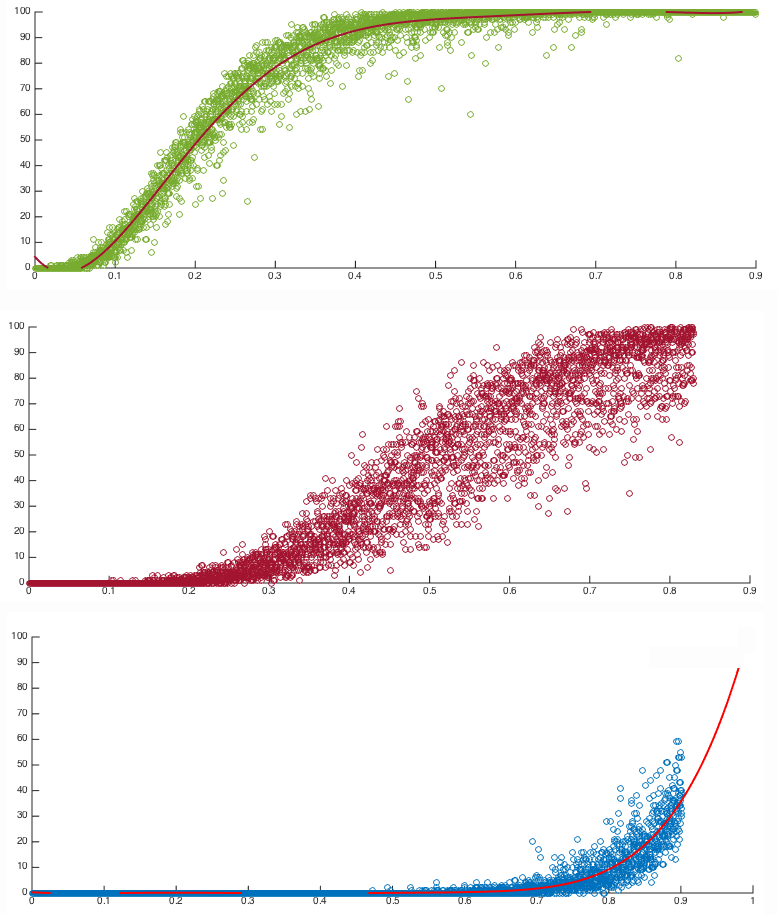
\includegraphics[scale=0.5]{imgs/RandSim1.png}
\end{center}
\caption[Probability distribution of a random node being an elite]{Simulation on a randomly generated network giving the probability of being an elite on the $y$-axis and the proportion of affiliations connected to on the $x$-axis. In all simulations the number of affiliations is 50. The top panel has 5 aspects; the middle panel has 10 aspects; and the bottom panel has 30 aspects.}
\label{RandSim1}
\end{figure}

\section[Additional information on data and regression analysis]{Additional information on data and regression analysis} \label{AppB}

Table~\ref{fin-ss} provides some summary statistics regarding all important variables used in the regression analysis throughout the econometric analysis in Section~\ref{Application:Regression}.

\begin{table}[h!]
\centering
\begin{tabular}{lccccc}
\\[-1.8ex]\hline
\hline \\[-1.8ex]
Statistic & \multicolumn{1}{c}{N} & \multicolumn{1}{c}{Mean} & \multicolumn{1}{c}{St. Dev.} & \multicolumn{1}{c}{Min} & \multicolumn{1}{c}{Max} \\
\hline \\[-1.8ex]
Profits ($\pi_{i}$) & 121 & 0.694 & 1.046 & 0.004 & 32 \\
Size ($\nu_{i}$) & 210 & 19.147 & 24.164 & 0.200 & 202.816 \\
Liquid & 174 & 1.536 & 3.811 & 0.000 & 27.753 \\
Illiquid & 174 & 6.813 & 13.722 & 0.001 & 85.937 \\
\begin{tabular}[c]{@{}l@{}}Interbank\\ borrowing\end{tabular} & 125 & 4.084 & 8.946 & 0.000 & 45.617 \\
\begin{tabular}[c]{@{}l@{}}Interbank\\ lending\end{tabular} & 174 & 1.202 & 1.789 & 0.000 & 12.568 \\
Years & 210 & 32.319 & 24.447 & 0 & 103 \\
Directors & 210 & 15.729 & 5.949 & 5 & 43 \\
$\sigma_{i}$ & 210 & 0.010 & 0.015 & 0.0001 & 0.088 \\
ExInf & 210 & 106,010,348 & 187,855,204 & 0.000 & 1,118,208,807 \\
Elites & 210 & 0.719 & 1.587 & 0 & 11 \\
$\delta_{i}$ & 210 & 15.514 & 15.206 & 0 & 71 \\
Weighted $\delta_{i}$ & 210 & 22.229 & 24.493 & 0 & 132 \\
Cluster & 210 & 0.336 & 0.246 & 0.000 & 1.000 \\
PageRank & 210 & 0.004 & 0.002 & 0.001 & 0.012 \\
Close & 210 & 0.371 & 0.101 & 0.000 & 0.522 \\
Between & 210 & 0.006 & 0.007 & 0.000 & 0.034 \\
Eigenvector & 210 & 0.173 & 0.226 & 0.000 & 0.965 \\
Beta & 210 & 0.925 & 0.647 & 0.000 & 3.111 \\
NatBanks & 210 & 3.129 & 3.383 & 0 & 16 \\
StateBank & 210 & 2.443 & 2.430 & 0 & 11 \\
SavingBank & 210 & 1.700 & 1.622 & 0 & 7 \\
Trusts & 210 & 4.348 & 4.578 & 0 & 21 \\
Railroad & 210 & 2.362 & 4.117 & 0 & 19 \\
Insurance & 210 & 1.533 & 1.998 & 0 & 8 \\
StateDum & 210 & 0.300 & 0.459 & 0 & 1 \\
NatDum & 210 & 0.233 & 0.424 & 0 & 1 \\
SavingsDum & 210 & 0.243 & 0.430 & 0 & 1 \\
TrustDum & 210 & 0.224 & 0.418 & 0 & 1 \\
BronxDum & 210 & 0.010 & 0.097 & 0 & 1 \\
BrooklynDum & 210 & 0.214 & 0.411 & 0 & 1 \\
ManhatDum & 210 & 0.690 & 0.463 & 0 & 1 \\
QueensDum & 210 & 0.038 & 0.192 & 0 & 1 \\
StatenDum & 210 & 0.019 & 0.137 & 0 & 1 \\
\hline \\[-1.8ex]
\end{tabular}
\label{fin-ss}
\caption{Summary statistics of important variables}
\end{table}

Table~\ref{profit-type-location} shows the regression results of profit and centrality where there are firm-type and location dummies.

\begin{table}[h!]
\centering
  \resizebox{\textwidth}{!}{%
\begin{tabular}{@{\extracolsep{5pt}}lD{.}{.}{-3} D{.}{.}{-3} D{.}{.}{-3} D{.}{.}{-3} D{.}{.}{-3} D{.}{.}{-3} }
\\[-1.8ex]\hline
\hline \\[-1.8ex]
 & \multicolumn{6}{c}{\textit{Dependent variable:}} \\
\cline{2-7}
\\[-1.8ex] & \multicolumn{6}{c}{Profit ($\pi_{i}$)} \\
\\[-1.8ex] & \multicolumn{1}{c}{(1)} & \multicolumn{1}{c}{(2)} & \multicolumn{1}{c}{(3)} & \multicolumn{1}{c}{(4)} & \multicolumn{1}{c}{(5)} & \multicolumn{1}{c}{(6)}\\
\hline \\[-1.8ex]
 Liquid & 0.129^{***} & 0.135^{***} & 0.134^{***} & 0.134^{***} & 0.133^{***} & 0.133^{***} \\
  & (0.017) & (0.018) & (0.018) & (0.018) & (0.018) & (0.018) \\
  Illiquid & -0.003 & 0.006 & 0.004 & 0.002 & 0.006 & 0.004 \\
  & (0.013) & (0.013) & (0.013) & (0.013) & (0.013) & (0.013) \\
  IBL & 0.068^{**} & 0.058 & 0.059 & 0.068^{*} & 0.054 & 0.063^{*} \\
  & (0.034) & (0.036) & (0.037) & (0.036) & (0.036) & (0.037) \\
  Years2 & 0.0001^{**} & 0.0001^{***} & 0.0001^{***} & 0.0001^{***} & 0.0001^{***} & 0.0001^{***} \\
  & (0.00003) & (0.00003) & (0.00003) & (0.00003) & (0.00003) & (0.00003) \\
  NumDir & -0.020 & -0.014 & -0.014 & -0.021 & -0.012 & -0.017 \\
  & (0.015) & (0.016) & (0.016) & (0.016) & (0.016) & (0.017) \\
  StateDum & -0.041 & -0.078 & -0.057 & -0.054 & -0.077 & -0.053 \\
  & (0.212) & (0.222) & (0.224) & (0.220) & (0.224) & (0.224) \\
  NatDum & -0.459^{**} & -0.483^{**} & -0.484^{**} & -0.491^{**} & -0.489^{**} & -0.490^{**} \\
  & (0.212) & (0.222) & (0.223) & (0.219) & (0.223) & (0.223) \\
  Railroad & -0.069^{**} & 0.003 & 0.013 & -0.014 & 0.032 & 0.019 \\
  & (0.031) & (0.024) & (0.023) & (0.023) & (0.030) & (0.014) \\
  BronxDum & -0.737 & -0.714 & -0.742 & -0.727 & -0.737 & -0.766 \\
  & (0.521) & (0.546) & (0.547) & (0.538) & (0.547) & (0.547) \\
  BrooklynDum & -0.311 & -0.287 & -0.301 & -0.321 & -0.280 & -0.313 \\
  & (0.346) & (0.362) & (0.364) & (0.358) & (0.364) & (0.364) \\
  ManhatDum & -0.433 & -0.481 & -0.540 & -0.510 & -0.511 & -0.535 \\
  & (0.337) & (0.355) & (0.355) & (0.348) & (0.355) & (0.353) \\
  QueensDum & -0.351 & -0.372 & -0.385 & -0.336 & -0.371 & -0.353 \\
  & (0.510) & (0.534) & (0.536) & (0.528) & (0.537) & (0.537) \\
  StatenDum & -0.199 & -0.237 & -0.244 & -0.170 & -0.268 & -0.232 \\
  & (0.637) & (0.668) & (0.671) & (0.661) & (0.670) & (0.670) \\
  $\sigma_{i}$ & 28.877^{***} &  &  &  &  &  \\
  & (8.791) &  &  &  &  &  \\
  Elite &  & 0.055 &  &  &  &  \\
  &  & (0.057) &  &  &  &  \\
  $\delta_{i}$ &  &  & 0.004 &  &  &  \\
  &  &  & (0.008) &  &  &  \\
  Weighted $\delta_{i}$ &  &  &  & 0.008^{*} &  &  \\
  &  &  &  & (0.004) &  &  \\
  Eigenvector &  &  &  &  & -0.212 &  \\
  &  &  &  &  & (0.598) &  \\
  $\beta_{i}$ &  &  &  &  &  & 0.078 \\
  &  &  &  &  &  & (0.113) \\
  Constant & 0.980^{**} & 0.953^{**} & 0.955^{**} & 0.967^{**} & 0.957^{**} & 0.963^{**} \\
  & (0.432) & (0.452) & (0.454) & (0.447) & (0.454) & (0.454) \\
 \hline \\[-1.8ex]
Observations & \multicolumn{1}{c}{117} & \multicolumn{1}{c}{117} & \multicolumn{1}{c}{117} & \multicolumn{1}{c}{117} & \multicolumn{1}{c}{117} & \multicolumn{1}{c}{117} \\
R$^{2}$ & \multicolumn{1}{c}{0.684} & \multicolumn{1}{c}{0.654} & \multicolumn{1}{c}{0.651} & \multicolumn{1}{c}{0.662} & \multicolumn{1}{c}{0.651} & \multicolumn{1}{c}{0.652} \\
Adjusted R$^{2}$ & \multicolumn{1}{c}{0.641} & \multicolumn{1}{c}{0.606} & \multicolumn{1}{c}{0.603} & \multicolumn{1}{c}{0.616} & \multicolumn{1}{c}{0.603} & \multicolumn{1}{c}{0.604} \\
\hline
\hline \\[-1.8ex]
\textit{Note:}  & \multicolumn{6}{r}{$^{*}$p$<$0.1; $^{**}$p$<$0.05; $^{***}$p$<$0.01} \\
\end{tabular}
}
\caption{Results of Profit-Centrality regressions with firm type and location dummies}
\label{profit-type-location}
\end{table}

Table~\ref{profit-interlock-type} shows the regression results of profit and centrality where the interlock types of each firm are categorised.

\begin{table}[h!]
\centering
  \resizebox{\textwidth}{!}{%
\begin{tabular}{@{\extracolsep{5pt}}lD{.}{.}{-3} D{.}{.}{-3} D{.}{.}{-3} D{.}{.}{-3} D{.}{.}{-3} D{.}{.}{-3} D{.}{.}{-3} }
\\[-1.8ex]\hline
\hline \\[-1.8ex]
 & \multicolumn{7}{c}{\textit{Dependent variable:}} \\
\cline{2-8}
\\[-1.8ex] & \multicolumn{7}{c}{Profit ($\pi_{i}$)} \\
\\[-1.8ex] & \multicolumn{1}{c}{(1)} & \multicolumn{1}{c}{(2)} & \multicolumn{1}{c}{(3)} & \multicolumn{1}{c}{(4)} & \multicolumn{1}{c}{(5)} & \multicolumn{1}{c}{(6)} & \multicolumn{1}{c}{(7)}\\
\hline \\[-1.8ex]
 Liquid & 0.106^{***} & 0.109^{***} & 0.104^{***} & 0.108^{***} & 0.104^{***} & 0.104^{***} & 0.104^{***} \\
  & (0.017) & (0.018) & (0.018) & (0.017) & (0.018) & (0.018) & (0.018) \\
  Illiquid & 0.004 & 0.014 & 0.014 & 0.011 & 0.013 & 0.015 & 0.014 \\
  & (0.013) & (0.014) & (0.014) & (0.013) & (0.014) & (0.014) & (0.014) \\
  IBL & 0.046 & 0.038 & 0.030 & 0.050 & 0.031 & 0.028 & 0.030 \\
  & (0.034) & (0.036) & (0.036) & (0.035) & (0.036) & (0.037) & (0.036) \\
  Years2 & 0.00004 & 0.0001^{**} & 0.0001^{**} & 0.0001^{**} & 0.0001^{**} & 0.0001^{*} & 0.0001^{**} \\
  & (0.00003) & (0.00003) & (0.00003) & (0.00003) & (0.00003) & (0.00003) & (0.00003) \\
  NumDir & -0.003 & 0.001 & 0.004 & -0.007 & 0.002 & 0.006 & 0.004 \\
  & (0.014) & (0.014) & (0.014) & (0.014) & (0.015) & (0.015) & (0.014) \\
  NatBanks & -0.042 & -0.054 & -0.037 & -0.069^{**} & -0.051 & -0.060 & -0.060^{*} \\
  & (0.035) & (0.036) & (0.071) & (0.034) & (0.042) & (0.036) & (0.036) \\
  StateBank & 0.021 & 0.042 & 0.070 & -0.006 & 0.046 & 0.053 & 0.047 \\
  & (0.033) & (0.033) & (0.064) & (0.036) & (0.033) & (0.038) & (0.033) \\
  SavingBank & 0.054 & 0.063 & 0.073 & 0.028 & 0.053 & 0.058 & 0.050 \\
  & (0.042) & (0.045) & (0.074) & (0.043) & (0.045) & (0.050) & (0.044) \\
  Trusts & -0.010 & -0.014 & 0.026 & -0.060^{**} & 0.014 & 0.003 & 0.003 \\
  & (0.022) & (0.025) & (0.071) & (0.029) & (0.032) & (0.022) & (0.022) \\
  Railroad & -0.047 & 0.019 & 0.071 & -0.021 & 0.065 & 0.048^{**} & 0.048^{**} \\
  & (0.036) & (0.030) & (0.067) & (0.030) & (0.044) & (0.022) & (0.022) \\
  Insurance & -0.024 & -0.014 &  & -0.048 & -0.010 & -0.022 & -0.023 \\
  & (0.054) & (0.056) &  & (0.054) & (0.064) & (0.057) & (0.056) \\
  Constant & 0.184 & 0.086 & 0.037 & 0.204 & 0.041 & 0.029 & 0.037 \\
  & (0.191) & (0.196) & (0.194) & (0.193) & (0.195) & (0.197) & (0.194) \\
  SigmaI & 30.457^{***} &  &  &  &  &  &  \\
  & (9.343) &  &  &  &  &  &  \\
  Elite &  & 0.096 &  &  &  &  &  \\
  &  & (0.065) &  &  &  &  &  \\
  D &  &  & -0.023 &  &  &  &  \\
  &  &  & (0.056) &  &  &  &  \\
  WD &  &  &  & 0.029^{***} &  &  &  \\
  &  &  &  & (0.009) &  &  &  \\
  Eigen &  &  &  &  & -0.716 &  &  \\
  &  &  &  &  & (1.559) &  &  \\
  Beta &  &  &  &  &  & -0.056 &  \\
  &  &  &  &  &  & (0.165) &  \\
 \hline \\[-1.8ex]
Observations & \multicolumn{1}{c}{117} & \multicolumn{1}{c}{117} & \multicolumn{1}{c}{117} & \multicolumn{1}{c}{117} & \multicolumn{1}{c}{117} & \multicolumn{1}{c}{117} & \multicolumn{1}{c}{117} \\
R$^{2}$ & \multicolumn{1}{c}{0.656} & \multicolumn{1}{c}{0.628} & \multicolumn{1}{c}{0.620} & \multicolumn{1}{c}{0.656} & \multicolumn{1}{c}{0.621} & \multicolumn{1}{c}{0.621} & \multicolumn{1}{c}{0.620} \\
Adjusted R$^{2}$ & \multicolumn{1}{c}{0.616} & \multicolumn{1}{c}{0.585} & \multicolumn{1}{c}{0.581} & \multicolumn{1}{c}{0.617} & \multicolumn{1}{c}{0.577} & \multicolumn{1}{c}{0.577} & \multicolumn{1}{c}{0.581} \\
\hline
\hline \\[-1.8ex]
\textit{Note:}  & \multicolumn{7}{r}{$^{*}$p$<$0.1; $^{**}$p$<$0.05; $^{***}$p$<$0.01} \\
\end{tabular}
}
\caption{Results of Profit-Centrality regressions with categorisation of interlocks}
\label{profit-interlock-type}
\end{table}


\section{Interlocking directorate formation} \label{AppD}

We provide a simple model of interlocking directorate formation on a weighted hypergraph. The weighted hypergraph consists of a set of nodes and a set of affiliations whereby each affiliation has a value attached. These concepts are defined above.

The primary goal of studying this model is to anticipate the structure of the directorate hypergraph and its network projections. Our specific interest is on the incentives of individual nodes in the formation of overlapping affiliations and the emergent structure from these incentives. From this we can give some insight regarding the connectivity of the directorate hypergraph and elite nodes, and can test the insights on the subsequent data analysis.

Within this formation situation individual nodes attempt to maximise their payoff and in doing so organise themselves into affiliations. In constructing the model we make a number of simplifying assumptions and argue their realism. First, we assume that each node is purely individualistic and, as a consequence, they do not consider the utilities of other agents; even those that operate in the same affiliation. Second, we argue that the utility of an individual node is derived directly from their influence in the hypergraph---which is well-defined by the $\sigma$-score---and indirectly from the influence of their neighbours. Third, we make the assumption that the inclusion of some node into an affiliation must benefit all incumbent members of the affiliation individually. Indeed, consent is required from all $i \in H$ so that $j \notin H$ can join $H$. Finally, we note that the indirect influence, or benefit, that some node $i \in N$ attains from a neighbour $j \in \overline{\Gamma}_{i}$ depends on the number of other neighbours $j$ has, and the relative weight of $i$'s connection to $j$.

\subsection{The interlocking directorate game}

The interlocking directorate game ($\mathcal{S}, \pi, N, \Gamma'$) is structured as a non-cooperative, strategic form game on some initial hypergraph structure $\Gamma'$ on node set $N = \{1,\ldots,n\}$, where $| \Gamma_{i} | = 1$ for all $i \in N$.

Nodes represent directors, or \emph{players}, who pursue the maximisation of both direct influence and indirect influence through their membership to affiliations and their subsequent neighbourhood. The hypergraph structure evolves from this initial setup to some stable state. The structure of the interlocking directorate game is given below.

\subsubsection*{Action sets}

Actions The action set for some player $i \in N$ is given by the following set of tuples:
\begin{equation}
\mathcal{S}_{i} = \left( \Gamma_{i} \times N \setminus \{i\} \right) \cup \left( \left( \Gamma \setminus \Gamma_{i} \right) \times \{i\} \right) ~ ,
\end{equation}
whereby $\Gamma_{i} \times N \setminus \{i\}$ refers to a set of potential \emph{requests} that $i$ can signal to other players to join any one of her affiliations $H \in \Gamma_{i}$, and $\left( \Gamma \setminus \Gamma_{i} \right) \times \{i\}$ refers to a set of \emph{responses} that $i$ can signal to other affiliations her willingness to join. Each player can choose to send a number of signals, such that the set of $i$'s signals is given by $S_{i} \subset \mathcal{S}_{i}$.

If $s_{i} = (H,j) \in S_{i}$ then player $i$ signals to all players in $H \in \Gamma_{i}$ her request for $j \notin H$ to participate in $H$. If $s_{i} = s_{k} = (H,j)$ for all $k \in H$ and $(H,j) \in S_{j}$ then $j$ will participate in $H$. Indeed, under this setting there is a requirement of consent whereby all $i \in H$ must benefit from $j$'s participation in $H$, and $j$ must also benefit from participating in $H$. We say that an action is \emph{stable} if and only if $s_{j} = (H,j)$ and $s_{i} = (H,j)$ for all $i \in H$.

\subsubsection*{Payoffs}

The payoff function of an individual node in a weighted hypergraph is formally given as:
\begin{equation} \label{payoff1}
\pi_{i}(\Gamma') = \sigma_{i}(\Gamma') + \sum_{j \in \overline{\Gamma}_{i}} a_{ij}(\Gamma') \sigma_{j}(\Gamma') ~ ,
\end{equation}
where:
\begin{equation}
a_{ij}(\Gamma') = \frac{\omega_{ij}^{\alpha}}{W_{j}(\Gamma')} ~ ,
\end{equation}
and:
\begin{equation}
\alpha = 1 - \frac{| \overline{\Gamma}_{i} \cap \overline{\Gamma}_{j} |}{| \overline{\Gamma}_{j} |} ~ .
\end{equation}
Note that for notational simplicity we let $\omega_{ij}(\Gamma') = \omega_{ij}$.

An individual player attains a payoff from a direct source and an indirect source. The direct source is from their own individual influence in the hypergraph, given by $\sigma_{i}(\Gamma')$. The indirect source refers to the influence of their neighbours, which is diluted by the proportional weight of the connection that $i$ has on her neighbour, thus $a_{ij}(\Gamma') \in [0,1]$.

The payoff from indirect influence is rationalised in two ways:
\begin{abet}
\item[(1)] Some $j \in \overline{\Gamma}_{i}$ can bring a new source of information to $i$. The amount useful information will be a function of $j$'s membership in the hypergraph, and thus can be captured by the $\sigma$-score; and

\item[(2)] Player $i$ may be able to provide $j$ information that $j$ can use to make decisions on; the impact of $i$'s information to $j$ will be captured by $i$'s relative access to $j$, given by $a_{ij}(\Gamma')$, and by $\sigma_{j}(\Gamma')$.
\end{abet}

Let $|H| = h$ for all $H \in \Gamma'$, such that $W_{j}(\Gamma) = \sum_{i \in \overline{\Gamma}_{j}} \omega_{ij} (\Gamma) = |\Gamma_{j}| \cdot (h-1)$. Moreover, if we let $\overline{\nu}_{H,i} = \frac{\sum_{H \in \Gamma_{i}} \nu_{H}}{| \Gamma_{i} |}$, then $\sigma_{i}(\Gamma) = |\Gamma_{i}| \cdot \frac{\overline{\nu}_{H,i}}{h}$. In doing this the payoff function becomes:
\begin{equation} \label{payoff2}
\pi_{i}(\Gamma') = | \Gamma_{i} | \cdot \left( \frac{\overline{\nu}_{H,i}}{h} \right) + \sum_{j \in \overline{\Gamma}_{i}} \frac{\omega_{ij}^{\alpha}}{(h-1)} \cdot \left( \frac{\overline{\nu}_{H,j}}{h} \right) ~ .
\end{equation}

%\paragraph{Some properties.}
%
%A number of properties can be determined from the utility function. First, the utility of an individual agent is always increasing with the number of affiliations that they are members of. Second, the utility of an individual agent is always decreasing as $h$ increases. Finally, $i$'s utility is increasing at a decreasing rate as more weight is placed on some $j$ if and only if $0 < \alpha < 1$. These points can be summarised with the following partial derivatives of the utility function
%\begin{align}
%\frac{\partial U_{i}(\Gamma)}{\partial |\Gamma_{i}|} & = \frac{\overline{\nu}_{H} \omega_{ij}^{\alpha}}{h-1} + \frac{\overline{\nu}_{H}}{h} ; \\
%\frac{\partial U_{i}(\Gamma)}{\partial h} & = - |\Gamma_{i}| \left( \frac{\overline{\nu}_{H} \omega_{ij}^{\alpha}}{(h-1)^2} + \frac{\overline{\nu}_{H}}{h^2} \right) ; \\
%\frac{\partial U_{i}(\Gamma)}{\partial h} & = \alpha |\Gamma_{i}| \frac{\overline{\nu}_{H} \omega_{ij}^{\alpha-1}}{h-1} . \\
%\end{align}

\subsection{Incentives and equilibrium analysis}

As the hypergraph evolves affiliations begin to overlap such that individual nodes become members of multiple affiliations. As noted from the action set the formation of overlapping affiliations requires consent from both parties involved.

The first party refers to the \emph{affiliations}: the set of nodes signalling to individual players their willingness for the player to join. The second party refers to the \emph{responders}: individual players signalling a response to the requests of affiliations. We define the incentives and decision-making processes of each party individually, and from this we assess the Strong Nash Equilibrium (SNE) of the interlocking game.

\subsubsection*{Incentives of the affiliations}

There exists a trade-off for each member of the affiliation, $i \in H$. The trade-off exists between reducing direct influence and increasing indirect influence by allowing $j$ to join the affiliation.

Formally, the loss to each $i \in H$ for allowing $j$ to join $H$ is given by:
\begin{equation}
\frac{\nu_{H}}{h} - \frac{\nu_{H}}{h+1} = - \frac{\nu_{H}}{h(h + 1)} ~ .
\end{equation}
The benefit to each $i \in H$ for allowing $j$ to join $H$ is given by:
\begin{equation}
\frac{(\omega_{ij}+1)^{\alpha}}{2h-1} \cdot \left( \frac{\overline{\nu}_{H',j}}{h} + \frac{\nu_{H}}{h+1} \right) - \frac{\omega_{ij}^{\alpha}}{(h-1)} \cdot \frac{\overline{\nu}_{H',j}}{h} ~ .
\end{equation}
If we allow $b_{ij} \cdot \nu_{H} = \overline{\nu}_{H',j}$, where $b_{ij} > 0$, then the decision for some $i \in H$ to signal to some $j \notin H$ to join affiliation $H$ is given by the inequality:
\begin{equation} \label{decisionfunction}
\frac{(\omega_{ij}+1)^{\alpha}}{2h-1} \cdot \left( \frac{\overline{\nu}_{H',j}}{h} + \frac{\nu_{H}}{h+1} \right) - \frac{\omega_{ij}^{\alpha}}{(h-1)} \cdot \frac{\overline{\nu}_{H',j}}{h} \geqslant \frac{\nu_{H}}{h(h + 1)} ~ .
\end{equation}

Player $j \notin H$ will be signalled by all members of $H$ if and only if the condition in Equation~\ref{decisionfunction} is satisfied for all $i \in H$. This will occur when $\overline{\nu}_{H',j} \geqslant b_{ij} \cdot \nu_{H}$. Solving for $b_{ij}$ in Equation~\ref{decisionfunction} we get:
\begin{equation} \label{eq:b}
b_{ij} \geqslant \frac{(h-1)(h((\omega_{ij} + 1)^{\alpha} - |\Gamma_{j}| - 1) + |\Gamma_{j}|)}{(h+1)(h((|\Gamma_{j}| + 1)\omega^{\alpha} - |\Gamma_{j}| (\omega_{ij} + 1)^{\alpha}) + |\Gamma_{j}|((\omega+1)^{\alpha} - \omega^{\alpha}))} ~ .
\end{equation}

Due to the characterisation of $\alpha$ there are diminishing returns for some $i \in H$ to signal to multiple $j \in H'$, or indeed strengthen the relation to some other $k \in H$.

\paragraph{Special cases.}

We note two special cases: one where $\omega_{ij} \geqslant 0$ and $\alpha = 1$; and the other where $\omega_{ij} = 0$ and $0 < \alpha < 1$. In these special cases the inequality in Equation~\ref{eq:b} simplifies to:
\begin{equation}
b \geqslant \frac{h - 1}{h + 1} ~ ,
\end{equation}
such that $b_{ij} = b$ for all $i \in H$ and all $j \notin H$.

Note that with the special cases the number of affiliations that $j$ is a member of, given by $| \Gamma_{j} |$, does not matter. Indeed, as $j$ becomes a member of more affiliations, the indirect influence of the node becomes increasingly diluted across more agents. Rather the only criteria must be that must be satisfied is that the average value of all affiliations that $j$ is a member of, given by $\overline{\nu}_{H',j}$, must be equal to or greater than $\left( \frac{h - 1}{h + 1} \right) \cdot \nu_{H}$, and thus $b \rightarrow 1$ as $h \rightarrow \infty$.

\subsubsection*{Incentives of responders}

From the payoff function we can see that a players' payoff is positively related to the number of affiliations that they are a member of. A players' direct influence increases with the number of affiliations. However, due to the unanimous consent required for membership into affiliation, becoming a member of affiliations with too low a value can lead to being rejected from affiliations that have a higher value.

Specifically, $(H',j) \in S_{j}$ if and only if:
\begin{equation} \label{eq:responder}
\frac{\sum_{H \in \Gamma_{j} \cup H'} \nu_{H}}{| \Gamma_{j} | + 1} \geqslant b_{ij} \cdot \nu_{H^{\star}} \mbox{ for all } i \in H^{\star} ~ ,
\end{equation}
where $H^{\star} \in \arg\max\{H \in \Gamma_{j} ~ | ~ \nu_{H} \geqslant \nu_{H'} \mbox{ for all } H' \in \Gamma_{j} \setminus H \}$.

In such a case player $j$ will only signal to affiliations that satisfy Equation~\ref{eq:responder}. Further, the responder will only accept signals from affiliations with the highest value, evaluating the affiliation with the next highest value with respect to Equation~\ref{eq:responder}, and so on until the equation cannot be satisfied for any other affiliation.

\paragraph{Special cases.}

With respect to the special cases noted above, since $b = b_{ij}$ for all $i \in H$, $(H,j) \in S_{j}$ if and only if:
\begin{equation}
\frac{\sum_{H \in \Gamma_{j} \cup H'} \nu_{H}}{| \Gamma_{j} | + 1} \geqslant \left( \frac{h - 1}{h + 1} \right) \cdot \nu_{H^{\star}} ~ .
\end{equation}

\paragraph{Concluding points.}

From this assessment we should find that, given a relatively high $h$, only affiliations of a similar value should have an overlapping directorates.
\begin{equation}
\frac{\sum_{H \in \Gamma_{j}} \nu_{H}}{| \Gamma_{j} |} \geqslant b_{ij} \cdot \nu_{H} \mbox{ for all } i,j \in H
\end{equation}

\end{subappendices}
